\documentclass[11pt,onecolumn]{article}
\usepackage{latexsym}
\usepackage{url}
\usepackage{float}
\usepackage{amsmath}
\usepackage{algpseudocode}
\usepackage{algorithm}
\usepackage{geometry}
\usepackage{subfig}
\geometry{left=2.0cm,right=2.0cm, top=2.0cm, bottom=2.0cm}
\usepackage{fancyhdr}
\usepackage{longtable}
\usepackage{url}
\usepackage{leftidx}
\usepackage{graphicx,grffile}
\usepackage{epstopdf}
\usepackage{multirow,bigstrut}
\usepackage{booktabs}
\usepackage{amsmath}
\usepackage{subfig}
\usepackage{soul,color}
\renewcommand{\algorithmicrequire}{\textbf{Input:}}
\renewcommand{\algorithmicensure}{\textbf{Output:}}
\newcommand{\algorithmicbreak}{\textbf{break}}
%\usepackage{subcaption}
\usepackage{caption}
\newcommand\figref[1]{Figure \ref{#1}}
\linespread{1}
\author{shuang ao\\
}
\title{
\large\textbf{Distilling}
}
\frenchspacing
\begin{document}
\maketitle
\section{Background}
\textit{Distillation for domain adaptation} \cite{hinton2015distilling} and \textit{privileged information} \cite{vapnik2015learning} are two techniques that enable machines to learn from other machines. Both methods address the problem how to build a student model that can learn from the advanced teacher models. Recently, Lopez \textit{et al.} \cite{lopez2015unifying} proposed a framework called \textit{generalized distillation} that unifies both techniques and show that it can be applied in many scenarios.
\subsection{Privileged information}
In the original work of the privileged information \cite{vapnik2015learning}, the data can be represented as a collection of the triples:
\[\{\left(x_1,x_1^*,y_1\right),\left(x_2,x_2^*,y_2\right) \dots \left(x_n,x_n^*,y_n\right)\}\]
where each $(x_i,y_i)$ is a feature-label pair, and the novel element $x_i$ is additional information about the example $(x_i,y_i)$ provided by an intelligent teacher, such as to support the learning process. However, in the testing procedure, the learning machine is not able to obtain the privileged information from the teacher. Vapnik?s learning using privileged information is one example of what we call machines-teaching machines: the paradigm where machines learn from other machines, in addition to training data. 
\subsection{Distillation}
Distillation uses a simple (student) machine learns a complex task by imitating the solution of a flexible (teacher) machine. For a $c$-class scenario, distillation works as follow: consider the data
\[\{x_i,y_i\}_{i=1}^n, \qquad x\in R^d, y\in \Delta^c\]
where $\Delta^c$ is a $c$-dimensional probability vector. In traditional learning, we try to learn a function $f_t$ that:
\begin{equation}\label{eq:normal}
f_t=\underset{f_t \in \mathcal{F}_t}{\arg \min}\frac{1}{n}\sum_{i=1}^{n}\ell\left(y_i,\sigma(f_t(x_i))\right)+\Omega(||f_t||)
\end{equation}
here $\sigma$ is the softmax operation:
\[\sigma(z)_k=\frac{e^{z_k}}{\sum_{j=1}^{c}e^{z_j}}\]
and $\ell$ is the cross-entropy loss function:
\[\ell(y,\hat{y})=-\sum_{i=1}^{c}y_i\log\hat{y}_i\]
In distillation, we try to learn the student machine $f_s$ to imitate the teacher machine $f_t$. During the learning process, $f_s$ can receive the soft label $s_i$ from the teacher machine $f_t$ for each training example $x_i$.
\begin{equation}\label{eq:softmax_T}
s_i=\sigma(f_t(x_i)/T)
\end{equation}
where $T$ is the temperature for distillation. It is worthy to note that in distillation, $f_t$ can either be a single large complex neural network or an ensemble of some complex classifiers. We can see that the soft label $s_i$, which reveals the class dependency, is more informative than the class label $y_i$.

The student machine can be learned by:
\begin{equation}\label{eq:distill}
f_s=\underset{f_s \in \mathcal{F}_s}{\arg \min}\frac{1}{n}\sum_{i=1}^{n}\left[\lambda\ell\left(y_i,\sigma(f_s(x_i))\right)+(1-\lambda)\ell\left(s_i,\sigma(f_s(x_i))\right)\right]
\end{equation}
here, $\mathcal{F}_s$ is a simpler function class than $\mathcal{F}_t$ and $\lambda$ is the imitation parameter to balance the importance between the hard label $y_i$ and the soft label $s_i$. The temperature $T>0$ controls how do we want to smooth the probability from the teacher $f_t$. Higher temperature leads to softer label.

\subsection{Generalized distillation}
Generalized distillation (GD) tries to unify the two frameworks together while using the soft label as the privileged information. The process of generalized distillation is as follows:

\begin{enumerate}
\item Learn teacher ${f}_t$ using the input-output pairs $\{x^*_i,y_i\}_{i=1}^n$ and Eq. \ref{eq:normal}.
\item Compute teacher soft labels $s_i$, using the temperature parameter $T > 0$.
\item Learn the student ${f}_s$ using the pair $\{\left(x_i,y_i\right),\left(x_i,s_i\right)\}_{i=1}^n$ and imitation parameter $\lambda$.
\end{enumerate}

\section{Domain adaptation with distilling SVMs}

GD can be used in many scenario such as multi-task learning, semi-supervised learning and reinforcement learning. As generalized distillation only required for the training inputs $\{x_i,y_i\}_{i=1}^n$ and the output $s$ from the teacher function $f_t$, it can be naturally applied in domain adaptation, called \textit{Generalized Distillation Domain Adaptation} (\textbf{GDDA}), where the the source model can be used as the teacher to output the soft labels and the student model is the target model. 

Similar to GD, the process of GDDA is as follow:
\begin{enumerate}
	\item For a $N$-class classification problem, suppose we have the training data $\{x_i,y_i\}_{i=1}^L$ and $M-1$ source (teacher) models $\{f^*_j\}_{j=1}^{M-1}$.
	\item For each of the training example $x_i$ and each source model $f^*_j$, computer the corresponding $N$-dimensional soft label $y^*_{ij}$ with some temperature $T>0$.
	\item Learn the target model $f_t$ using the $(M+1)$-tuple $\{x_i,y_i,y^*_{i1},\dots,y^*_{M-1}\}_{i=1}^L$ with some imitation parameters $\{\lambda_i\}^M_{i=1}$
\end{enumerate} 

There are several advantages for applying generalized distillation for domain adaptation:
\begin{enumerate}
\item Compatible with \textbf{various of classifiers}. GD only requires the outputs of the teacher model instead of asking for the specific parameters of the teacher model. Therefore, we can treat the teacher model, either a single model (single source) or an ensemble of models (multi-source), as a black-box. This means GDDA is compatible with almost any types of source model.
\item Highly effective in \textbf{small data regimes}. The theoretical analysis shows that the teacher is most helpful when working with small datasets, or in the initial stages of online learning. In domain adaptation, we also requires to learn an effective target classifier with just a few training examples.
\item Compatible with \textbf{different scenarios}. GD can be used in a semi-supervised scenario. Similarly, GDDA can work in many different transfer learning scenarios besides a supervised setting. For example, in a unsupervised transfer learning scenario, we can set the imitation parameter of the hard label to 0 and learn the target model. In the semi-supervised scenario, we can choose a small value for the imitation parameter of the hard label as it could be less informative than the soft labels. 
%a semi-supervised scenario and utilize the soft label of the unlabeled data to further improve performance of the target model. 
\item \textbf{Better generalization performance}. According to GD, the student model can be a much simple function than the teacher model. This implies that the VC dimension of the student model is smaller than the teacher(s). According to the principle of Empirical Risk Minimization (EMR) \cite{vapnik1999overview}, in GDDA, as long as the student (target) model achieves the same training error of the teacher (source) model(s), it should have better generalization ability. This means the knowledge of the source model(s) can be effective transferred to the target task.
\end{enumerate}

In GDDA, we have to decide the values of 2 parameters, the temperature $T$ and imitation parameter $\lambda$. The temperature $T$ control the smoothness of the soft label and the imitation parameter $\lambda$ controls how similar the target model is to the source model. It is obvious that the value of imitation parameter can greatly affect the performance of the target model and choosing a proper imitation parameter can greatly improve the transfer efficiency. In the previous work of GD, the imitation parameter is determined by brute force search which greatly reduces its effectiveness. In domain adaptation, it is common that there could be multiple source models to be exploited and it is tedious to search the imitation parameter for each of the source model.

To solve this problem, we propose a novel method that can determined the imitation parameter $\lambda$ autonomously, called GDDA-SVM. In our GDDA-SVM, instead of using cross-entropy loss, we use Mean Squared Error (MSE) as our loss function for the following two reasons: (1) Some recently work \cite{ba2014deep} \cite{luo2016face} \cite{romero2014fitnets} \cite{urban2016deep} show that MSE is also an efficient measurement for a student model to mimic the behavior of the teacher model. (2) MSE can provide a closed form cross-validation error estimation and help us to choose the proper imitation parameter effectively. 



%\subsection{GDDA-SVM} 
%\begin{equation}
\begin{aligned}
\min \qquad & L = \frac{1}{2}{\left| w \right|^2} + C \lambda \sum\limits_i {e_{1,i}^2}  + C \left( {1 - \lambda } \right)\sum\limits_i {e_{2,i}^2} \\
s.t.\qquad& e_{1,i} = y_i - wx_i\\
& e_{2,i} = s_i - wx_i\\
& \lambda \in [0,1]
\end{aligned}  
\end{equation}
Lagrangian:
\begin{equation}
L = \frac{1}{2}{\left| w \right|^2} + C[\lambda \sum\limits_i {e_{1,i}^2}  + \left( {1 - \lambda } \right)\sum\limits_i {e_{2,i}^2}]  + \sum\limits_i {{\alpha _i}\left( {y_i - wx_i - {e_{1,i}}} \right)}  + \sum\limits_i {{\beta _i}\left( {s_i - wx_i - {e_{2,i}}} \right)} 
\end{equation}
derivative:
\begin{equation}
\begin{aligned}
\frac{{\partial L}}{{\partial w}}& = w - \sum\limits_i {\left( {{\alpha _i} + {\beta _i}} \right)} {x_i}=0 \rightarrow w = \sum\limits_i {\left( {{\alpha _i} + {\beta _i}} \right)} {x_i}\\
\frac{{\partial L}}{{\partial {e_{1,i}}}} & = 2C\lambda {e_{1,i}} - {\alpha _i}=0 \rightarrow \alpha_i = 2C\lambda {e_{1,i}}\\
\frac{{\partial L}}{{\partial {e_{2,i}}}}&= 2C\left( {1 - \lambda } \right){e_{2,i}} - {\beta _i}=0 \rightarrow \beta_i = 2C(1-\lambda)e_{2,i}\\
\end{aligned}
\end{equation}
let $K$ be the kernel matrix:
\begin{equation}
\begin{aligned}
K(\alpha+\beta)+\frac{\mathbf{I}}{2C\lambda}\alpha&=Y\\
K(\alpha+\beta)+\frac{\mathbf{I}}{2C(1-\lambda)}\beta&=S
\end{aligned}
\end{equation}
Sum up:
\begin{equation}
\begin{aligned}
\frac{K(\alpha+\beta)}{(1-\lambda)}+\frac{\mathbf{I}}{2C\lambda(1-\lambda)}\alpha&=\frac{Y}{(1-\lambda) }\\
\frac{K(\alpha+\beta)}{\lambda}+\frac{\mathbf{I}}{2C (1-\lambda)\lambda}\beta&=\frac{S}{\lambda}\\
\frac{K(\alpha+\beta)}{\lambda(1-\lambda)}+\frac{\mathbf{I}(\beta+\alpha)}{2C(1-\lambda)\lambda}&=\frac{S}{\lambda}+\frac{Y}{1-\lambda}\\
[K+\frac{\mathbf{I}}{2C}][\beta+\alpha]&=(1-\lambda)S+\lambda Y
\end{aligned}
\end{equation}
let $M=[K+\frac{\mathbf{I}}{2C}]$, $\eta = [\alpha+\beta]$, $\eta'= M^{-1}Y$,$\eta''= M^{-1}S$
we have:
\[\eta = (1-\lambda)\eta''+\lambda\eta'\]
According to \cite{cawley2006leave}, the Leave-one-out error of the model for example $x_i$ is:
\[\lambda Y_i + (1-\lambda)S_i-\hat{Y_i} = (1-\lambda)\frac{\eta_i''}{M_{ii}^{-1}}+\lambda\frac{\eta_i'}{M_{ii}^{-1}}\]
\[\hat{Y_i}(\lambda) = (S_i-\frac{\eta_i''}{{M_{ii}^{-1}}})+\lambda\left(Y_i-S_i+\frac{\eta_i''}{M_{ii}^{-1}}-\frac{\eta_i'}{M_{ii}^{-1}}\right)\]
\subsection{Multi-class Loss}
We use two kinds of loss function for multi-class: hinge loss and cross-entropy
\subsubsection{Multi-class hinge loss}
For multi-class, $i$ denotes the instance id and $j$ denotes the class id:
\begin{equation}
\hat{Y_{ij}}(\lambda) = (S_{ij}-\frac{\eta_{ij}''}{{M_{ii}^{-1}}})+\lambda\left(Y_{ij}-S_{ij}+\frac{\eta_{ij}''}{M_{ii}^{-1}}-\frac{\eta_{ij}'}{M_{ii}^{-1}}\right)
\end{equation}
Let 
\[\mu_{ij} = \left(Y_{ij}-S_{ij}+\frac{\eta_{ij}''}{M_{ii}^{-1}}-\frac{\eta_{ij}'}{M_{ii}^{-1}}\right) \]
and
\[b_{ij}=S_{ij}-\frac{\eta_{ij}''}{{M_{ii}^{-1}}}\]
\begin{equation}
L_{h}\left( {\lambda ,i} \right) = \mathop {\max }\limits_r {\left[ {1 - {\varepsilon _{r,{y_i}}} + {{\hat Y}_{ir}}\left( {\lambda } \right) - {{\hat Y}_{i{y_i}}}\left( {\lambda } \right)} \right]}
\end{equation}
\begin{equation}
\begin{aligned}
\frac{\partial L_h^{(i)}}{\partial \lambda}&= 
\begin{cases}
0 & L_h^{(i)}=0\\
\mu_{i,r}-\mu_{i,y_i}& \text{otherwise}
\end{cases}\\
\end{aligned}
\end{equation}
\subsubsection{Categorical Cross-entropy}
With softmax activation:
\begin{equation}
\begin{aligned}
P_{ij} &= \frac{e^{\hat{Y}_{ij}/T}}{\sum_{h} e^{\hat{Y}_{ih}/T}}\\
L_{c}\left( {\lambda ,i} \right) &= -\sum_{j}Y_{ij}\log\left({P_{ij}}(\lambda)\right)\\
\frac{\partial L_c^{(i)}}{\partial \hat{Y}_{ij}}&=\left(P_{ij}-Y_{ij}\right)
\end{aligned}
\end{equation}

\[\frac{\partial L_c^{(i)}}{\partial \lambda}=\sum_{j}\mu_{ij}\left(P_{ij}-Y_{ij}\right)\]

\subsection{Distillation with multiple sources}
Suppose we have $L$ examples $\{x_i,y_i\}_{i=1}^L$ from and $N$ classes where $X\in R^{L\times d}, Y\in R^{L\times N}$. Meanwhile, there are $M-1$ the source (teacher) models providing the soft labels $\{Y^*_i\}_{i=1}^{M-1}$ for each of the $L$ examples. As 
Combining the hard label $Y$ and soft label $Y^*$, we have our new label matrix: $S = R^{M\times L \times N}$. To solve this $N$-class classification problem, we adopt the One-vs-All strategy to build $N$ binary SVMs.
To obtain the $n$th binary SVM, we have to solve the following optimization problem: 
\begin{equation}\label{eq:multi-distill}
\begin{aligned}
\min \qquad & \frac{1}{2}{\left| w_n \right|^2} + C\sum_{i,j} \lambda_i{e_{ijn}^2} \\
s.t.\qquad& e_{ijn} = s_{ijn} - w_nx_j\\
& \sum_i\lambda_i=1\\
& \lambda \in [0,1]; i\in M;  j\in L\\
\end{aligned}  
\end{equation}
To solve this optimization problem, we use KKT theorem \cite{cristianini2000introduction} and add the dual sets of variables to the Lagrangian of the optimization problem:
\begin{equation}
\mathcal{L}=\frac{1}{2}{\left| w_n \right|^2} + C\sum_{i,j} \lambda_i{e_{ijn}^2}+\sum_{i,j}\alpha^{(n)}_{ij}\left(s_{ij} - wx_j-e_{ij}\right)+\beta^{(n)}\left(\sum_i\lambda_i-1\right)
\end{equation}
To find the saddle point, 
\begin{equation}
\begin{aligned}
\frac{{\partial L}}{{\partial w_n}}& = w_n - \sum_{j}\alpha^{(n)}_{ij} {x_j}=0 \rightarrow w_n = \sum_{j}\alpha^{(n)}_{ij} {x_j}\\
\frac{{\partial L}}{{\partial {e_{ijn}}}} & = 2C\lambda_i {e_{ijn}} - {\alpha^{(n)} _{ij}}=0 \rightarrow \alpha^{(n)}_{ij} = 2C\lambda_i {e_{ijn}}\\
\end{aligned}
\end{equation}
For each example $x_j$ and its constraint of label $s_{ijn}$, we have $e_{ijn}  + w_nx_j= s_{ijn}$. Replacing $w_n$ and $e_{ijn}$,  we have:  
\begin{equation}
\begin{aligned}
%x_j\sum_{k}\alpha^{(n)}_{ik}x_k+\frac{\alpha^{(n)}_{ij}}{2C\lambda_i}&=s_{ijn}\\
\lambda_ix_j\sum_{k}\alpha^{(n)}_{ik}x_k+\frac{\alpha^{(n)}_{ij}}{2C}&=\lambda_is_{ijn}
%x_j\sum_{k}\alpha^{(n)}_{ik}x_k+\sum_j\frac{\alpha^{(n)}_{ij}}{2C}&=\sum_j\lambda_js_{ijn}
\end{aligned}
\end{equation}
Summing over each constraint of example $x_j$, we have:
\begin{equation}
\underbrace{\sum_i\lambda_i}_{=1} x_j\sum_{k}\alpha^{(n)}_{ik}x_k+\sum_i\frac{\alpha^{(n)}_{ij}}{2C}=\sum_i\lambda_is_{ijn}
\end{equation}
%Here we use $K$ to denote the kernel matrix $K=\{x_ix_j|i,j\in 1\dots L\}$.
Let %$M=[K+\frac{\mathbf{I}}{2C}]$ and 
$\eta_{jn}=\sum_i\alpha^{(n)}_{ij}$, we have:
\begin{equation}
\begin{aligned}
\sum_j\eta_{jn}x_jx_i+\frac{\eta_{in}}{2C}&=\sum_i\lambda_is_{ijn}\\
%M\eta_n&=S_n\begin{bmatrix}
%\lambda_1\\\vdots\\\lambda_m
%\end{bmatrix}
\end{aligned}
\end{equation}

This implies that solving the optimization problem \eqref{eq:multi-distill} is equivalent to solve a standard LS-SVM whose the target is encoded as $\sum_i\lambda_is_{ijn}$, i.e. the weighted label matrix $S$.

Here we use $\Omega$ to denote the matrix $\Omega=[K+\frac{\mathbf{I}}{2C}]$ where $K$ is the kernel matrix $K=\{x_ix_j|i,j\in 1\dots L\}$. To simplify our notation, let ${\eta}'_{n}=M^{-1}S_n$ where $S_n$ is the matrix $S_n=\{s_{ijn}|i\in M;j\in L\}$ and $\Omega^{-1}$ is the inverse of matrix $\Omega$. 
\[\eta_{jn}=\sum_i\lambda_i{\eta}'_{ijn}\]

The Leave-one-out estimation of the example $x_j$ for the $n$th binary SVM can be written as \cite{cawley2006leave}:
\[\sum_i\lambda_is_{ijn}-\hat{y}_{jn} =\frac{{\eta}_{jn}}{\Omega_{jj}^{-1}} =\frac{\sum_i\lambda_i{\eta}'_{ijn}}{\Omega_{jj}^{-1}}\]
\begin{equation}\label{eq:yhat}
\hat{y}_{jn} = \sum_i\lambda_i\left(s_{ijn}-\frac{{\eta}'_{ijn}}{\Omega_{jj}^{-1}}\right)
\end{equation}
where $\Omega^{-1}_{jj}$ is the $j$th diagonal element of $\Omega^{-1}$. Now, we have found an efficient way to estimate the output of each binary student model for example $x_j$. In the following part, we will introduce how to find the optimal $\lambda_i$ for each of the source models. 
\subsection{Cross-entropy loss for imitation parameter estimation}
From the previous part, we have already found a effective way to estimate the output of the SVM. The optimal imitation parameters, can be found by solving the following optimization problem:
\begin{equation}
\begin{aligned}
\min \quad& L_c\left(\lambda\right)=\frac{1}{2}\sum_i^M||\lambda_i||^2+\frac{1}{L}\sum_{j,n}\ell\left(y_{in},\hat{y}_{jn}\left(\lambda\right)\right)
\end{aligned}
\end{equation}
Here we use the L2 regularization term to guarantee that the estimated $\lambda$ can perform well on the testing data. For the loss $\ell(\cdot)$, We choose the cross-entropy (CE) as the loss function.
Compared to MSE, cross-entropy pay less attention to a single incorrect predicted example which reduced the affect of the outlier example in the training data. Moreover, cross-entropy works better with unlabeled data. Assume that we use one-hot strategy to encode the hard labels of the labeled examples while encoding the unlabeled examples with all 0s. When we use cross-entropy, no loss with generate from the side of the hard labels for the unlabeled examples. The target model only simulate the outputs from the source models. Therefore, 
Let:
\begin{equation}\label{eq:mu}
\mu_{ijn}=s_{ijn}-\frac{{\eta}'_{ijn}}{\Omega_{jj}^{-1}}
\end{equation}
\begin{equation}
P_{jn} = \frac{e^{\hat{y}_{jn}}}{\sum_{h} e^{\hat{y}_{jh}}}
\end{equation}
\begin{equation}\label{eq:p}
\begin{aligned}
\frac{\partial \ell(\lambda)}{\partial \lambda_i}&=\sum_n\mu_{ijn}\left(P_{jn}-{y}_{jn}\right)
\end{aligned}
\end{equation}

\begin{algorithm}
	\caption{GDDA-SVM}
	\begin{algorithmic}
		\Require Input examples $X=\{x_1,...,x_L\}$, number of classes $N$, size of sources $M$, 3D label matrix, $S=[Y_1,Y_2,...,Y_{M}]$ with size $L\times M \times N$, temperature $T$, optimization iteration $iter$
		\Ensure Target model $f_t = Wx$
		\State Compute $\Omega=[K+\frac{\mathbf{I}}{2C}]$
		\State Compute imitation parameter $\lambda$ with Algorithm \ref{alg:lambda}
		\State Compute new label $Y_{new}=\sum_i\lambda_iY_i$
		\State Compute $\eta = \Omega^{-1}Y_{new}$
		\State Compute $w_n = \sum_j \eta_{jn}x_j$
	\end{algorithmic}	
\end{algorithm}

\begin{algorithm}
	\caption{$\lambda$ Optimization}\label{alg:lambda}
\begin{algorithmic}
	\Require Input examples $X$, number of classes $N$, size of sources $M$, 3D label matrix $S$, temperature $T$, optimization iteration $iter$, Kernel matrix $\Omega$
    \Ensure Imitation parameter $\lambda$
    \State Initialize $\lambda = \frac{1}{M}$, 
    
    \State Let $S_n$ be the label matrix of $S$ for class $n$
    \For{Each label $S_n$} 
    \State Compute $\eta'_n=\Omega^{-1}S_n$ 
    \EndFor
    \State Compute $\mu$ using \eqref{eq:mu}
    \For {$it \in iter$ }
	    \State Compute $\hat{y}_{jn}$ and $P_{jn}$ with \eqref{eq:yhat}  and \eqref{eq:p}
	    \State $\Delta_{\lambda} \leftarrow 0$
	    \For {each $x_j$ in $X$}
		    \State $\Delta_{\lambda} = \Delta_{\lambda}+\sum_n\mu_{ijn}\left(P_{jn}-{y}_{jn}\right)$
	    \EndFor
	    \State $\Delta_{\lambda} =\Delta_{\lambda}/L$
	    \State $\lambda = \lambda - \frac{1}{itr}(\Delta_{\lambda}+\lambda)$
    \EndFor
\end{algorithmic}	
\end{algorithm}





\subsection{Distillation with multiple sources}
Suppose we have $L$ examples $\{x_i,y_i\}_{i=1}^L$ from and $N$ classes where $X\in R^{L\times d}, Y\in R^{L\times N}$. Meanwhile, there are $M-1$ the source (teacher) models providing the soft labels $\{Y^*_i\}_{i=1}^{M-1}$ for each of the $L$ examples. As 
Combining the hard label $Y$ and soft label $Y^*$, we have our new label matrix: $S = R^{M\times L \times N}$. To solve this $N$-class classification problem, we adopt the One-vs-All strategy to build $N$ binary SVMs.
To obtain the $n$th binary SVM, we have to solve the following optimization problem: 
\begin{equation}\label{eq:multi-distill}
\begin{aligned}
\min \qquad & \frac{1}{2}{\left| w_n \right|^2} + C\sum_{i,j} \lambda_i{e_{ijn}^2} \\
s.t.\qquad& e_{ijn} = s_{ijn} - w_nx_j\\
& \sum_i\lambda_i=1\\
& \lambda \in [0,1]; i\in M;  j\in L\\
\end{aligned}  
\end{equation}
To solve this optimization problem, we use KKT theorem \cite{cristianini2000introduction} and add the dual sets of variables to the Lagrangian of the optimization problem:
\begin{equation}
\mathcal{L}=\frac{1}{2}{\left| w_n \right|^2} + C\sum_{i,j} \lambda_i{e_{ijn}^2}+\sum_{i,j}\alpha^{(n)}_{ij}\left(s_{ij} - wx_j-e_{ij}\right)+\beta^{(n)}\left(\sum_i\lambda_i-1\right)
\end{equation}
To find the saddle point, 
\begin{equation}
\begin{aligned}
\frac{{\partial L}}{{\partial w_n}}& = w_n - \sum_{j}\alpha^{(n)}_{ij} {x_j}=0 \rightarrow w_n = \sum_{j}\alpha^{(n)}_{ij} {x_j}\\
\frac{{\partial L}}{{\partial {e_{ijn}}}} & = 2C\lambda_i {e_{ijn}} - {\alpha^{(n)} _{ij}}=0 \rightarrow \alpha^{(n)}_{ij} = 2C\lambda_i {e_{ijn}}\\
\end{aligned}
\end{equation}
For each example $x_j$ and its constraint of label $s_{ijn}$, we have $e_{ijn}  + w_nx_j= s_{ijn}$. Replacing $w_n$ and $e_{ijn}$,  we have:  
\begin{equation}
\begin{aligned}
%x_j\sum_{k}\alpha^{(n)}_{ik}x_k+\frac{\alpha^{(n)}_{ij}}{2C\lambda_i}&=s_{ijn}\\
\lambda_ix_j\sum_{k}\alpha^{(n)}_{ik}x_k+\frac{\alpha^{(n)}_{ij}}{2C}&=\lambda_is_{ijn}
%x_j\sum_{k}\alpha^{(n)}_{ik}x_k+\sum_j\frac{\alpha^{(n)}_{ij}}{2C}&=\sum_j\lambda_js_{ijn}
\end{aligned}
\end{equation}
Summing over each constraint of example $x_j$, we have:
\begin{equation}
\underbrace{\sum_i\lambda_i}_{=1} x_j\sum_{k}\alpha^{(n)}_{ik}x_k+\sum_i\frac{\alpha^{(n)}_{ij}}{2C}=\sum_i\lambda_is_{ijn}
\end{equation}
%Here we use $K$ to denote the kernel matrix $K=\{x_ix_j|i,j\in 1\dots L\}$.
Let %$M=[K+\frac{\mathbf{I}}{2C}]$ and 
$\eta_{jn}=\sum_i\alpha^{(n)}_{ij}$, we have:
\begin{equation}
\begin{aligned}
\sum_j\eta_{jn}x_jx_i+\frac{\eta_{in}}{2C}&=\sum_i\lambda_is_{ijn}\\
%M\eta_n&=S_n\begin{bmatrix}
%\lambda_1\\\vdots\\\lambda_m
%\end{bmatrix}
\end{aligned}
\end{equation}

This implies that solving the optimization problem \eqref{eq:multi-distill} is equivalent to solve a standard LS-SVM whose the target is encoded as $\sum_i\lambda_is_{ijn}$, i.e. the weighted label matrix $S$.

Here we use $\Omega$ to denote the matrix $\Omega=[K+\frac{\mathbf{I}}{2C}]$ where $K$ is the kernel matrix $K=\{x_ix_j|i,j\in 1\dots L\}$. To simplify our notation, let ${\eta}'_{n}=M^{-1}S_n$ where $S_n$ is the matrix $S_n=\{s_{ijn}|i\in M;j\in L\}$ and $\Omega^{-1}$ is the inverse of matrix $\Omega$. 
\[\eta_{jn}=\sum_i\lambda_i{\eta}'_{ijn}\]

The Leave-one-out estimation of the example $x_j$ for the $n$th binary SVM can be written as \cite{cawley2006leave}:
\[\sum_i\lambda_is_{ijn}-\hat{y}_{jn} =\frac{{\eta}_{jn}}{\Omega_{jj}^{-1}} =\frac{\sum_i\lambda_i{\eta}'_{ijn}}{\Omega_{jj}^{-1}}\]
\begin{equation}\label{eq:yhat}
\hat{y}_{jn} = \sum_i\lambda_i\left(s_{ijn}-\frac{{\eta}'_{ijn}}{\Omega_{jj}^{-1}}\right)
\end{equation}
where $\Omega^{-1}_{jj}$ is the $j$th diagonal element of $\Omega^{-1}$. Now, we have found an efficient way to estimate the output of each binary student model for example $x_j$. In the following part, we will introduce how to find the optimal $\lambda_i$ for each of the source models. 
\subsection{Cross-entropy loss for imitation parameter estimation}
From the previous part, we have already found a effective way to estimate the output of the SVM. The optimal imitation parameters, can be found by solving the following optimization problem:
\begin{equation}
\begin{aligned}
\min \quad& L_c\left(\lambda\right)=\frac{1}{2}\sum_i^M||\lambda_i||^2+\frac{1}{L}\sum_{j,n}\ell\left(y_{in},\hat{y}_{jn}\left(\lambda\right)\right)
\end{aligned}
\end{equation}
Here we use the L2 regularization term to guarantee that the estimated $\lambda$ can perform well on the testing data. For the loss $\ell(\cdot)$, We choose the cross-entropy (CE) as the loss function.
Compared to MSE, cross-entropy pay less attention to a single incorrect predicted example which reduced the affect of the outlier example in the training data. Moreover, cross-entropy works better with unlabeled data. Assume that we use one-hot strategy to encode the hard labels of the labeled examples while encoding the unlabeled examples with all 0s. When we use cross-entropy, no loss with generate from the side of the hard labels for the unlabeled examples. The target model only simulate the outputs from the source models. Therefore, 
Let:
\begin{equation}\label{eq:mu}
\mu_{ijn}=s_{ijn}-\frac{{\eta}'_{ijn}}{\Omega_{jj}^{-1}}
\end{equation}
\begin{equation}
P_{jn} = \frac{e^{\hat{y}_{jn}}}{\sum_{h} e^{\hat{y}_{jh}}}
\end{equation}
\begin{equation}\label{eq:p}
\begin{aligned}
\frac{\partial \ell(\lambda)}{\partial \lambda_i}&=\sum_n\mu_{ijn}\left(P_{jn}-{y}_{jn}\right)
\end{aligned}
\end{equation}

\begin{algorithm}
	\caption{GDDA-SVM}
	\begin{algorithmic}
		\Require Input examples $X=\{x_1,...,x_L\}$, number of classes $N$, size of sources $M$, 3D label matrix, $S=[Y_1,Y_2,...,Y_{M}]$ with size $L\times M \times N$, temperature $T$, optimization iteration $iter$
		\Ensure Target model $f_t = Wx$
		\State Compute $\Omega=[K+\frac{\mathbf{I}}{2C}]$
		\State Compute imitation parameter $\lambda$ with Algorithm \ref{alg:lambda}
		\State Compute new label $Y_{new}=\sum_i\lambda_iY_i$
		\State Compute $\eta = \Omega^{-1}Y_{new}$
		\State Compute $w_n = \sum_j \eta_{jn}x_j$
	\end{algorithmic}	
\end{algorithm}

\begin{algorithm}
	\caption{$\lambda$ Optimization}\label{alg:lambda}
\begin{algorithmic}
	\Require Input examples $X$, number of classes $N$, size of sources $M$, 3D label matrix $S$, temperature $T$, optimization iteration $iter$, Kernel matrix $\Omega$
    \Ensure Imitation parameter $\lambda$
    \State Initialize $\lambda = \frac{1}{M}$, 
    
    \State Let $S_n$ be the label matrix of $S$ for class $n$
    \For{Each label $S_n$} 
    \State Compute $\eta'_n=\Omega^{-1}S_n$ 
    \EndFor
    \State Compute $\mu$ using \eqref{eq:mu}
    \For {$it \in iter$ }
	    \State Compute $\hat{y}_{jn}$ and $P_{jn}$ with \eqref{eq:yhat}  and \eqref{eq:p}
	    \State $\Delta_{\lambda} \leftarrow 0$
	    \For {each $x_j$ in $X$}
		    \State $\Delta_{\lambda} = \Delta_{\lambda}+\sum_n\mu_{ijn}\left(P_{jn}-{y}_{jn}\right)$
	    \EndFor
	    \State $\Delta_{\lambda} =\Delta_{\lambda}/L$
	    \State $\lambda = \lambda - \frac{1}{itr}(\Delta_{\lambda}+\lambda)$
    \EndFor
\end{algorithmic}	
\end{algorithm}


\section{Experiments}
\subsection{Single Source for Office datasets}
There are 3 subsets in offices datasets, webcam (795), amazon (2817) and dslr (498), sharing 31 classes. We perform 2 adaptation experiments, transferring from webcam to amazon and from dslr to amazon. 

We use the features extracted from Alexnet \cite{KrizhevskyNIPS12} FC7 as the input features for both source and target domain. The teacher (source) model is trained with MLP on the whole source dataset and student (target) model is trained with GDDA-SVM. We also use brute force to search the imitation parameter $\lambda$ in range $[0,0.1,...,1]$ and show the results. Here our experiments run in a semi-supervised scenario where there are some unlabeled data in the target training set in each experiment. We also show the performance of the teacher model on the target task, denoted as "teacher". To avoid the randomness, we perform each experiments 10 times and report the results.
\newpage
\subsubsection{From DSLR to Amazon}
\begin{figure}[h]
\centering
\begin{tabular}{cc}
\subfloat[5 unlabeled ]{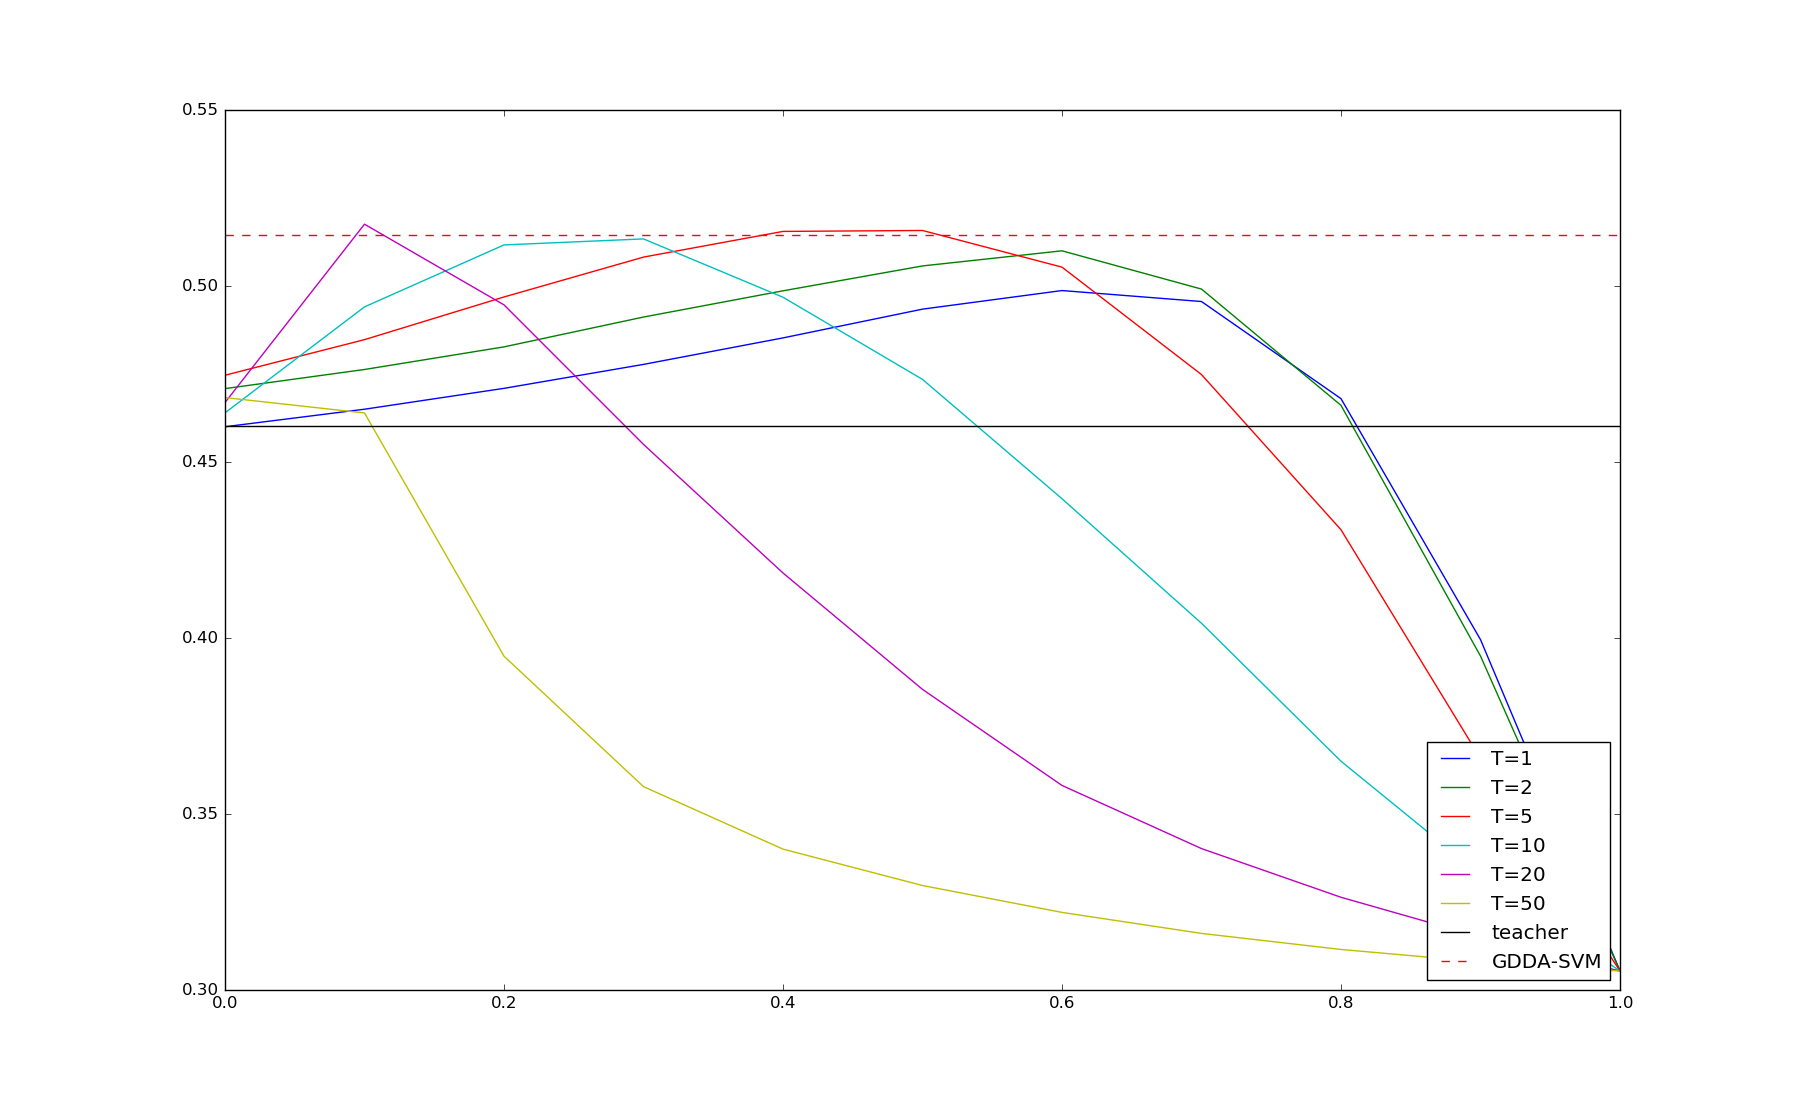
\includegraphics[width=0.45\textwidth]{figure/dslr1.png}}&
\subfloat[10 unlabeled]{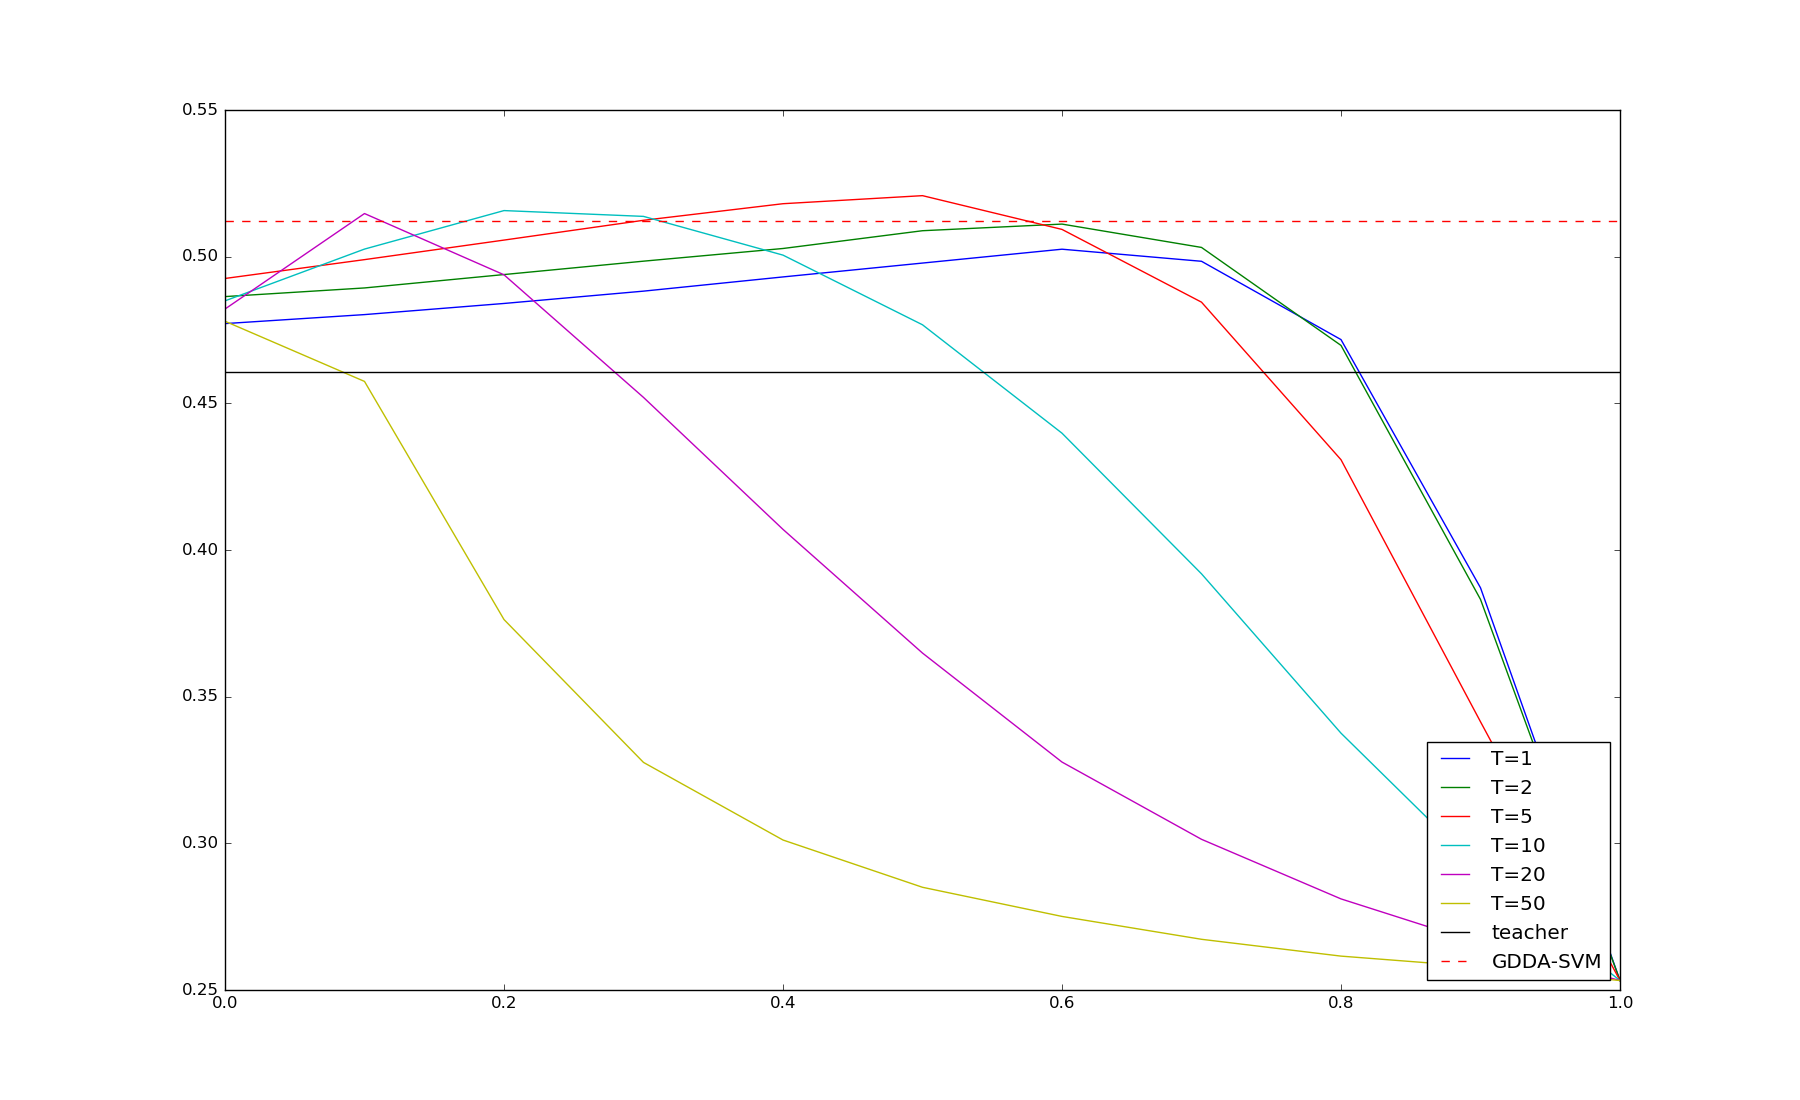
\includegraphics[width=0.45\textwidth]{figure/dslr2.png}}\\
\subfloat[15 unlabeled]{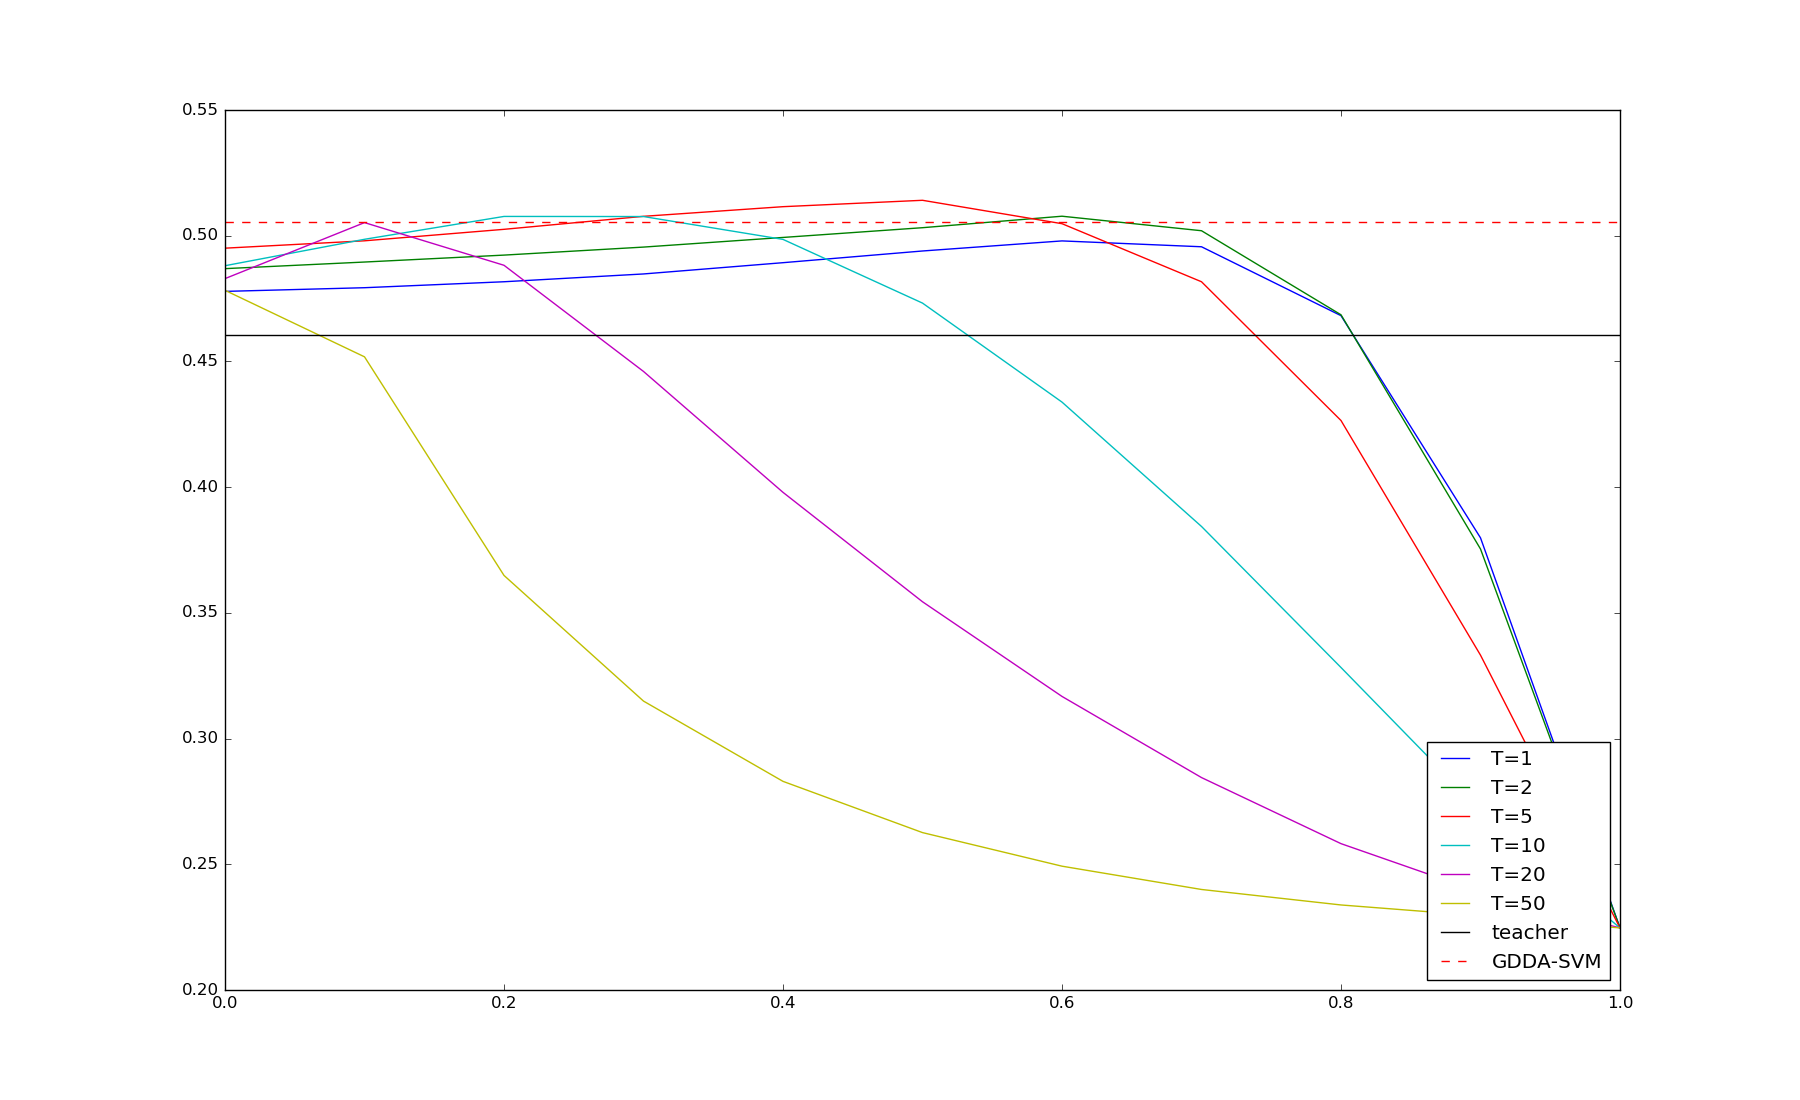
\includegraphics[width=0.45\textwidth]{figure/dslr3.png}}&
\subfloat[20 unlabeled]{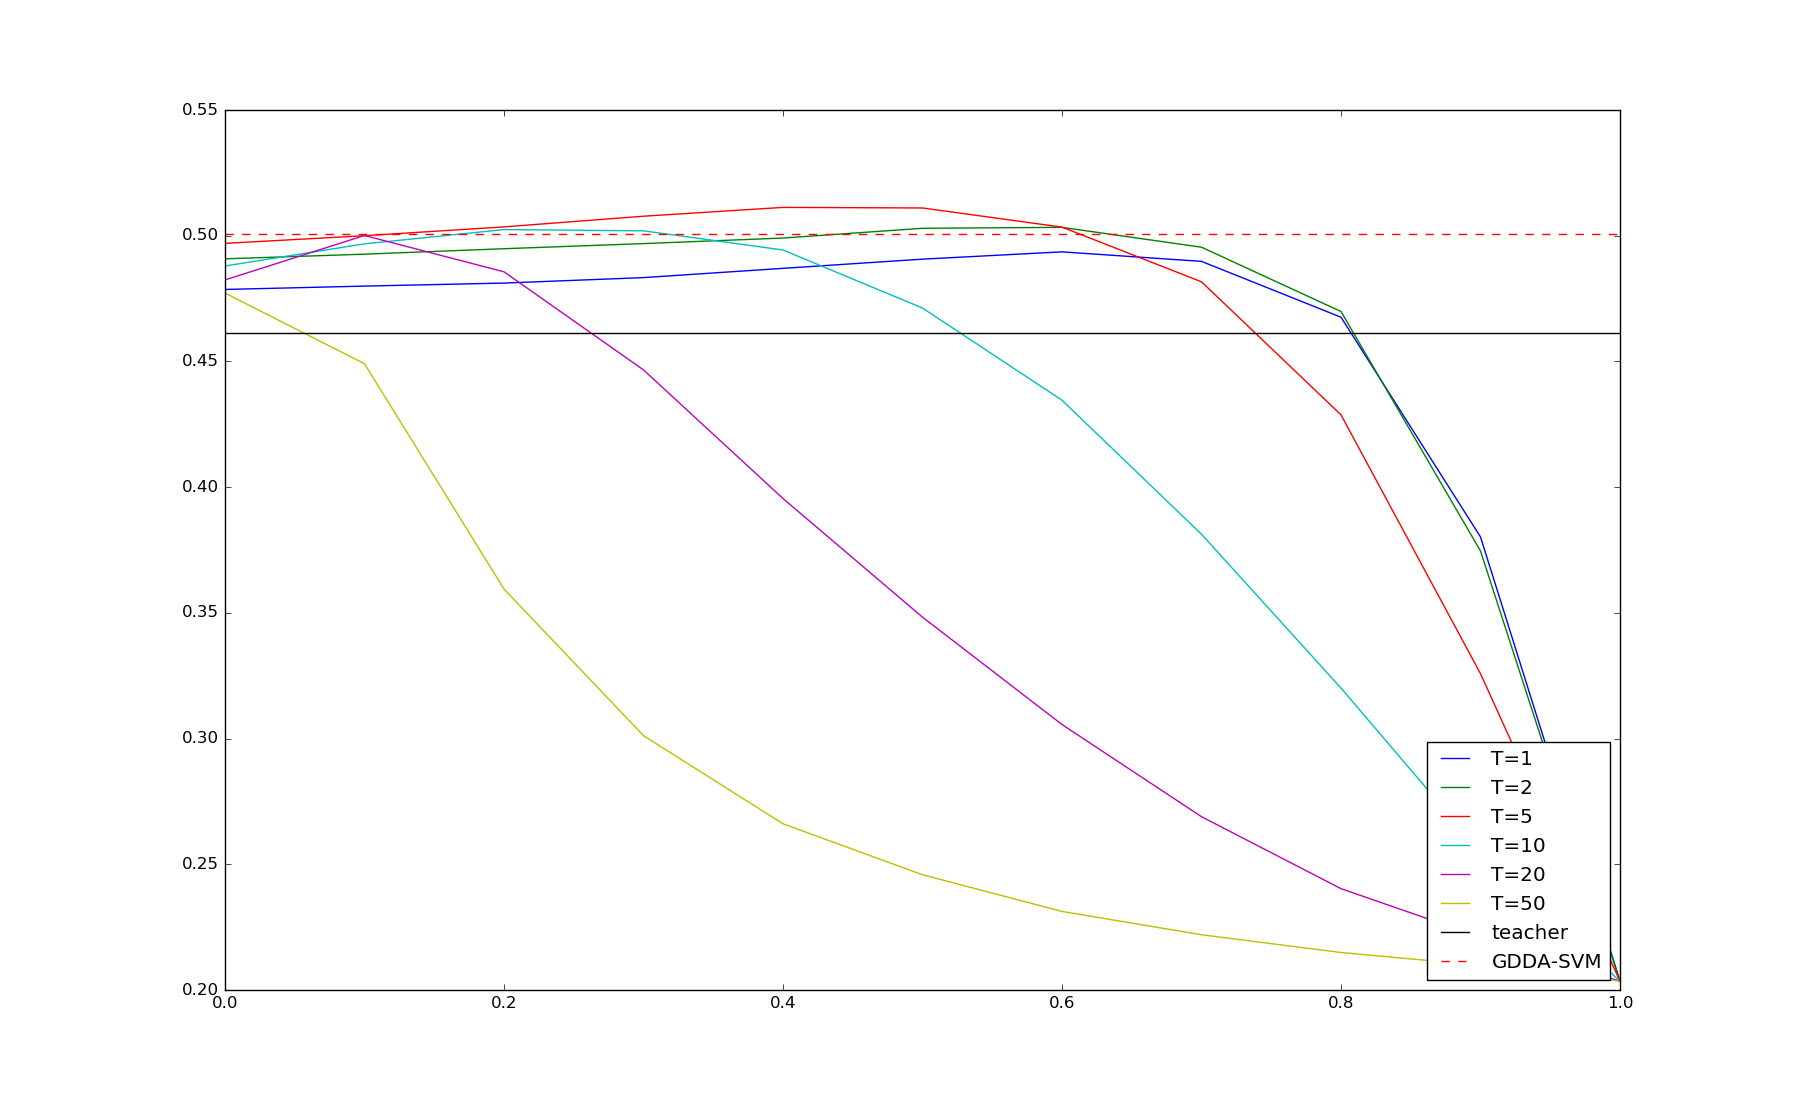
\includegraphics[width=0.45\textwidth]{figure/dslr4.png}}\\
\end{tabular}
\caption{DSLR $\rightarrow$ Amazon. Semi-supervised adaptation with one labeled instance per class.}
\end{figure}
\newpage
\subsubsection{From Webcam to Amazon}
\begin{figure}[h]
\centering
\begin{tabular}{cc}
\subfloat[5 unlabeled ]{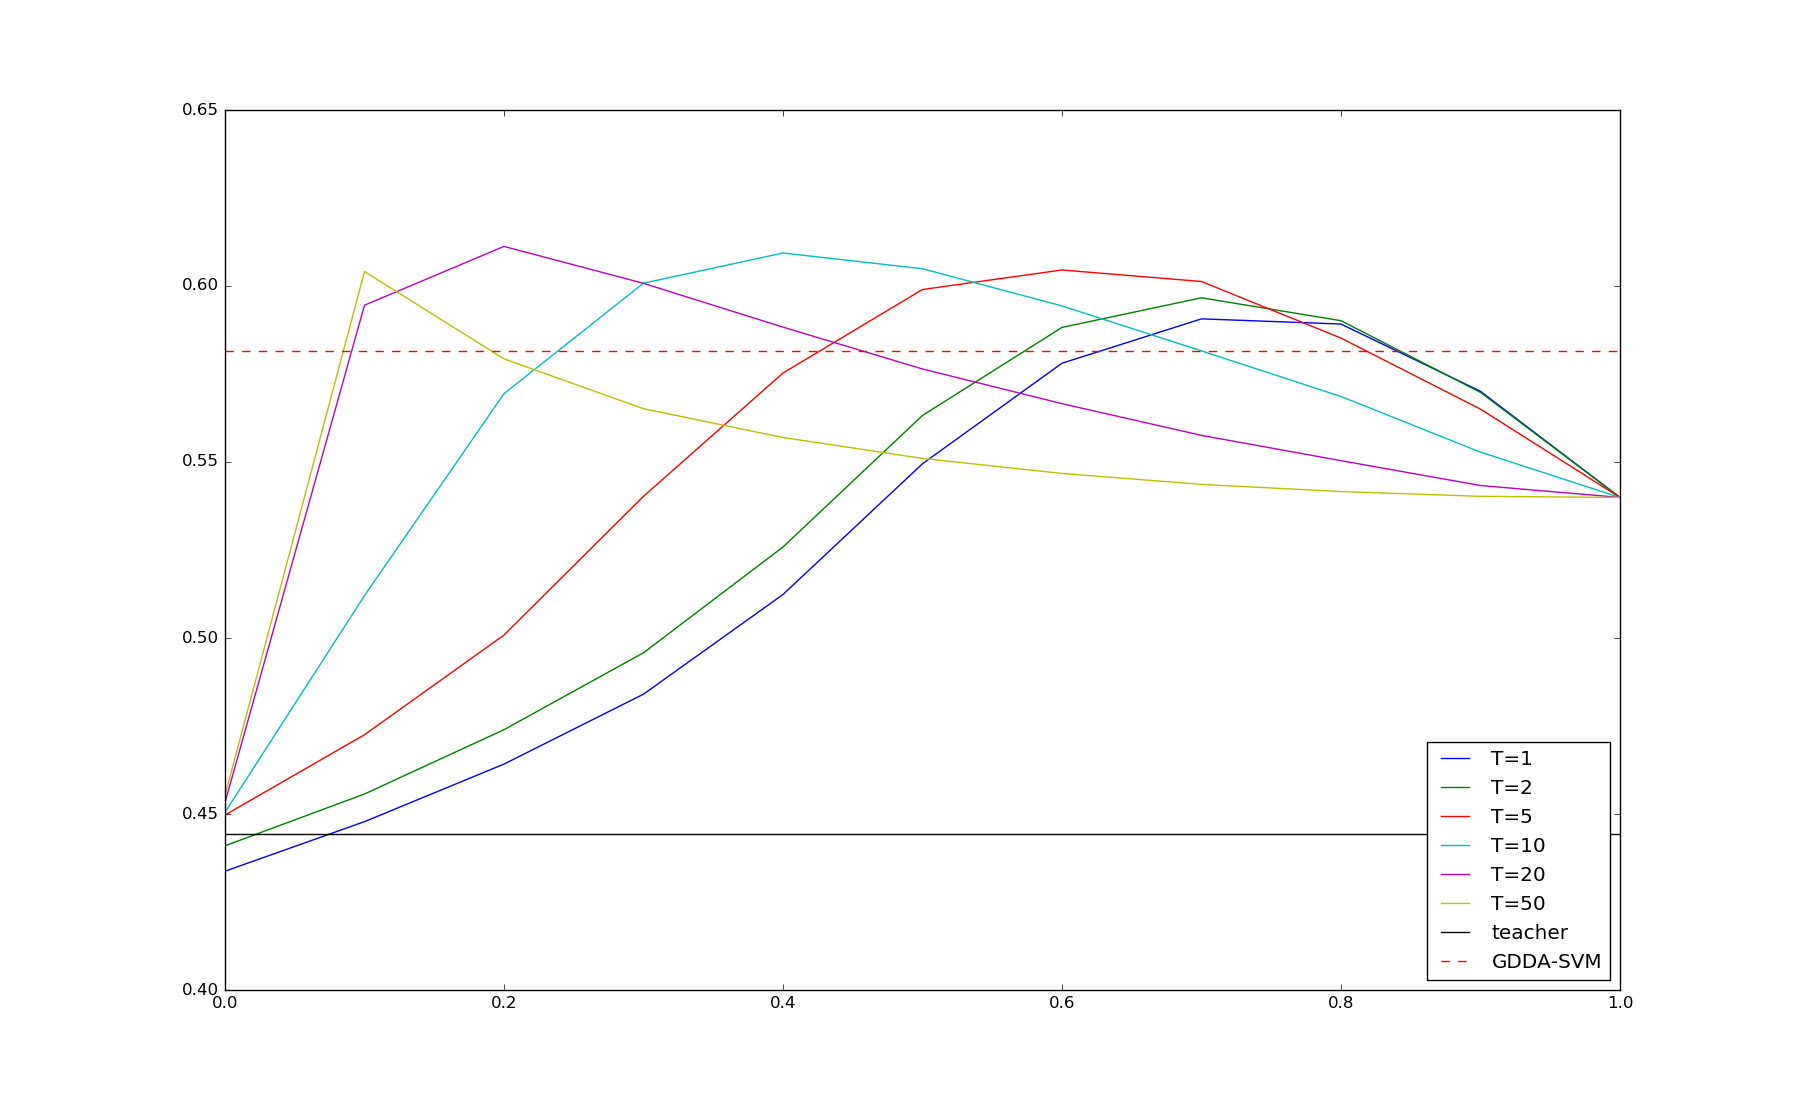
\includegraphics[width=0.45\textwidth]{figure/webcam1.png}}&
\subfloat[10 unlabeled]{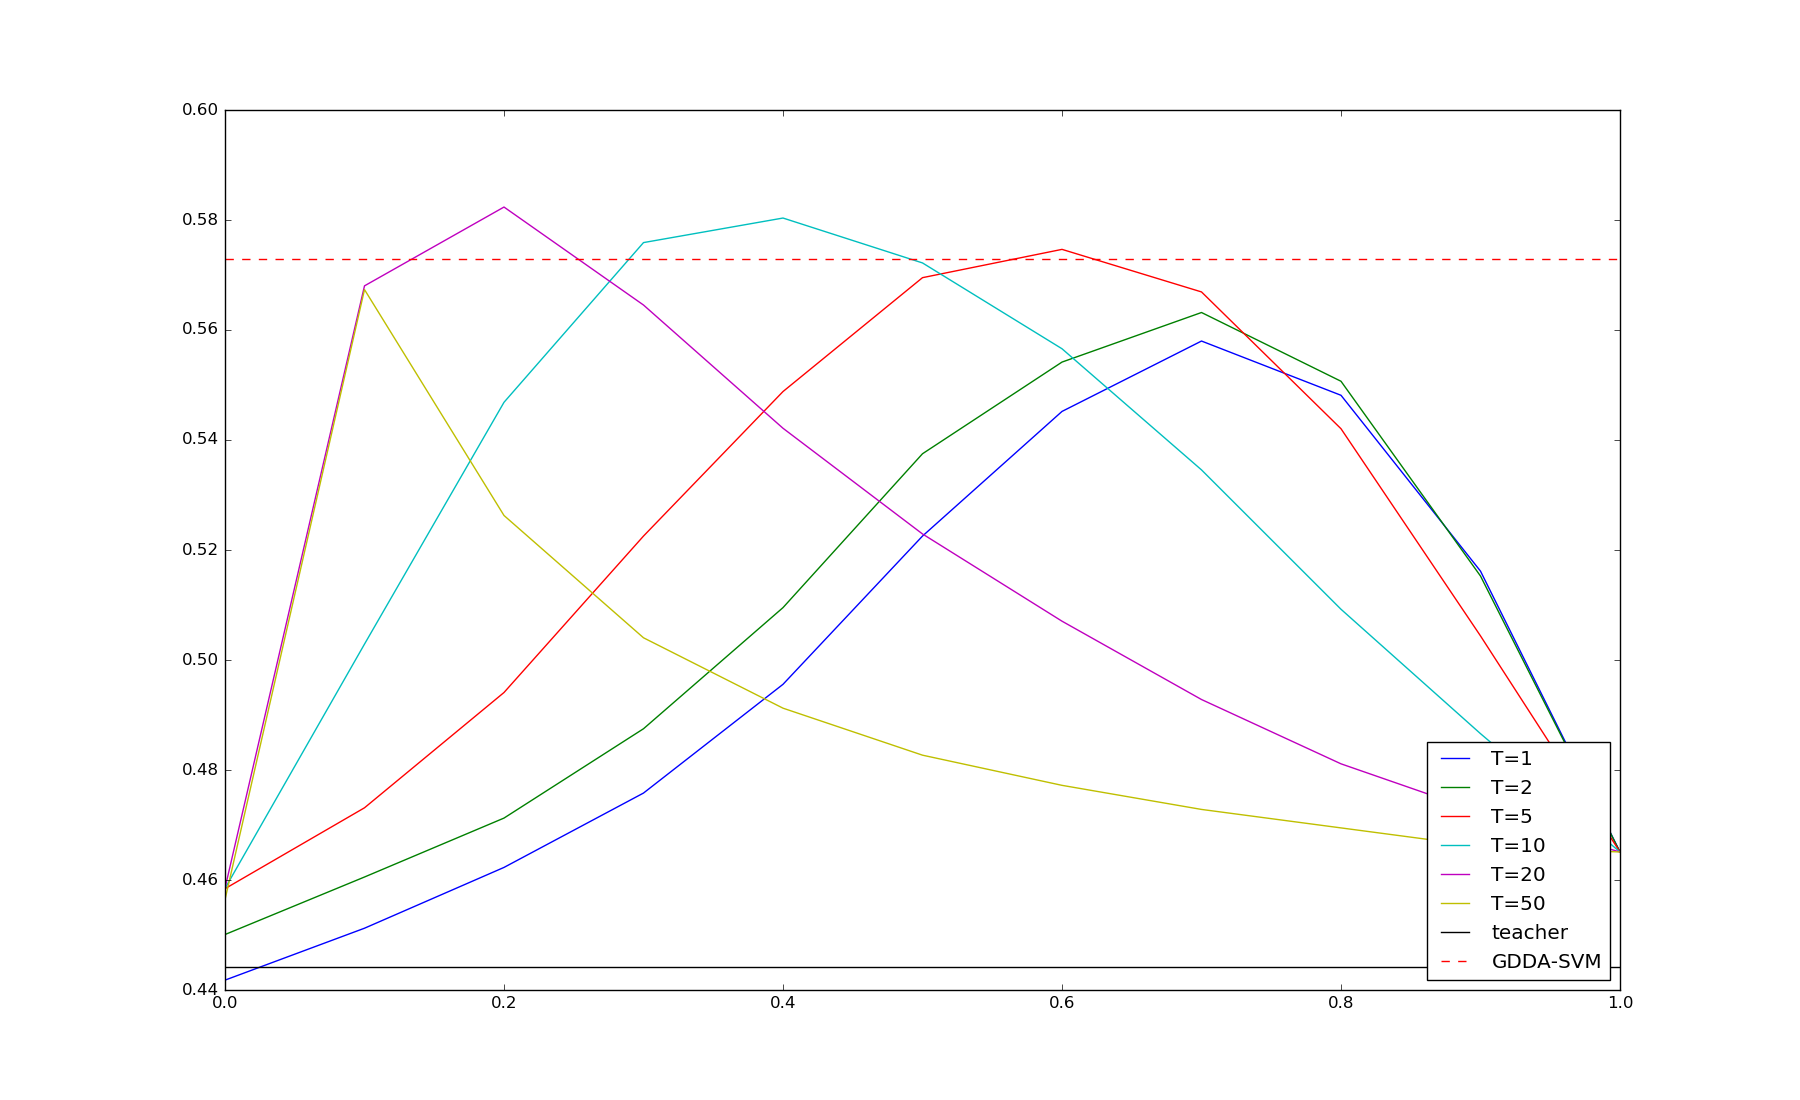
\includegraphics[width=0.45\textwidth]{figure/webcam2.png}}\\
\subfloat[15 unlabeled]{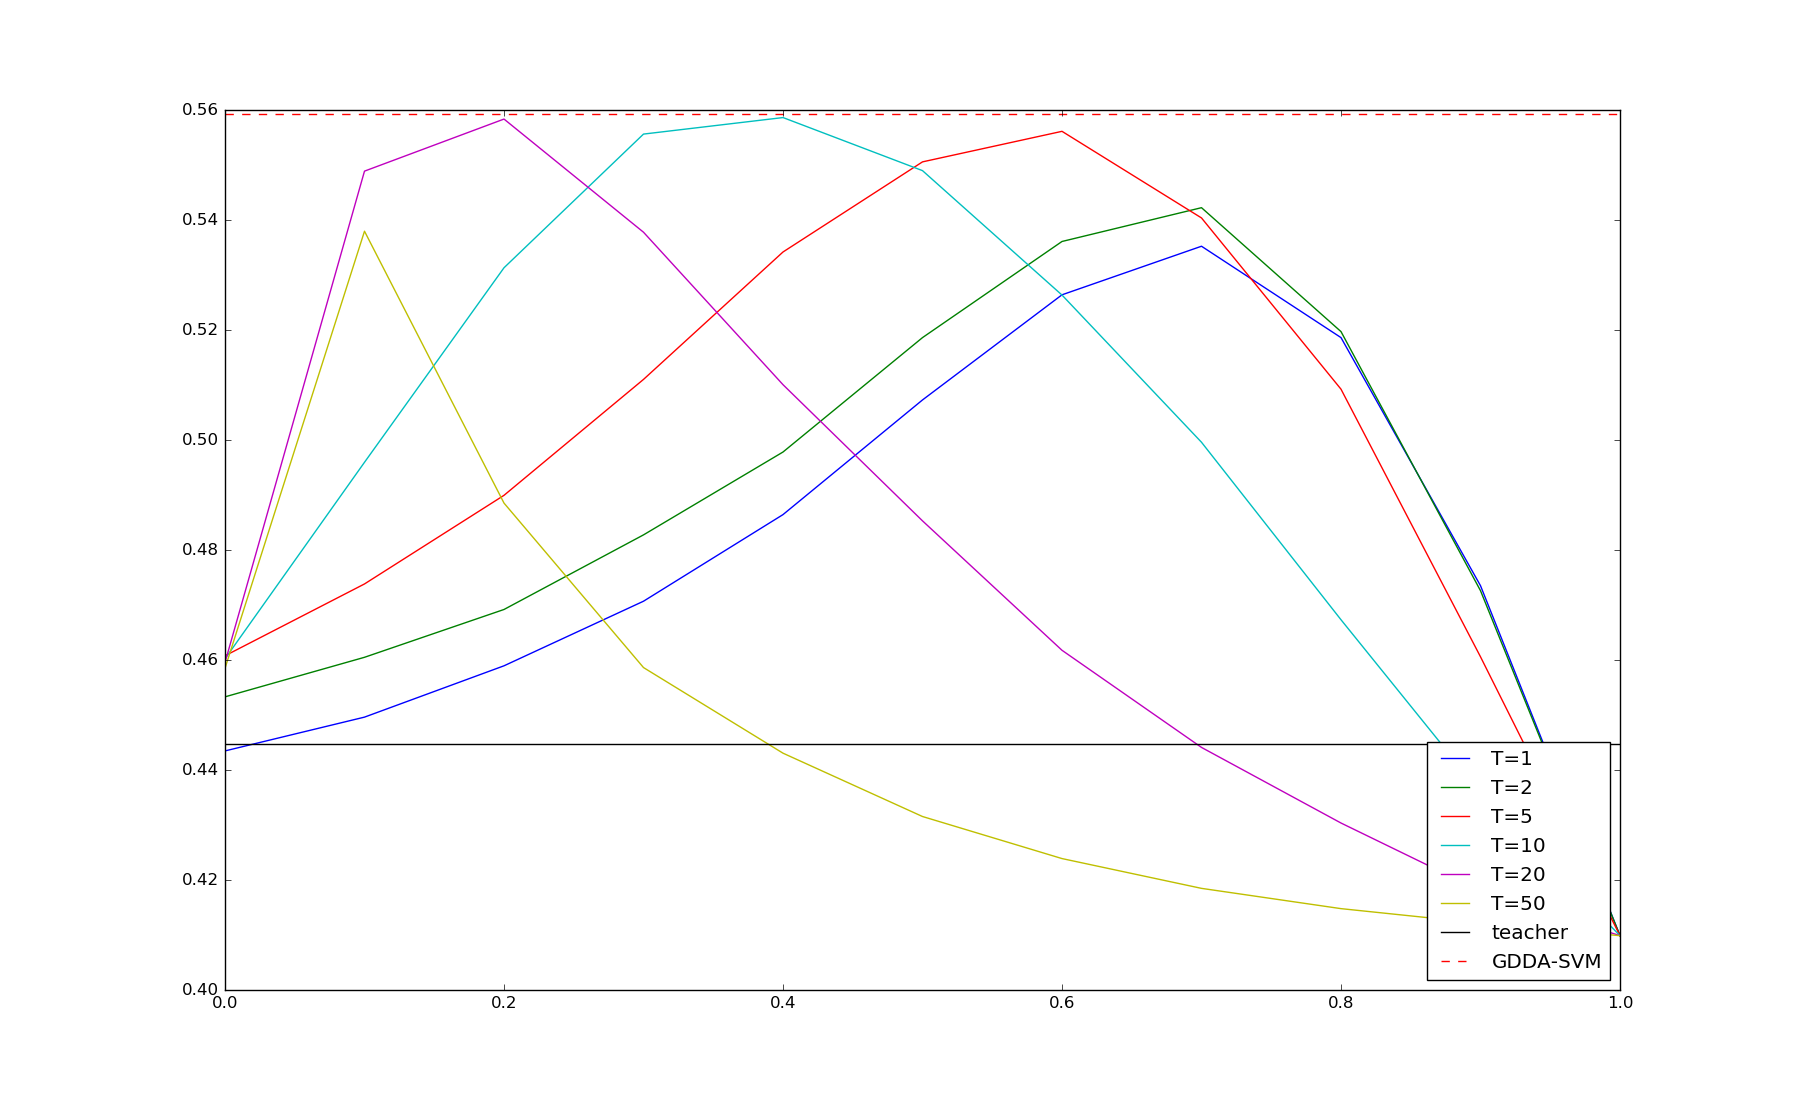
\includegraphics[width=0.45\textwidth]{figure/webcam3.png}}&
\subfloat[20 unlabeled]{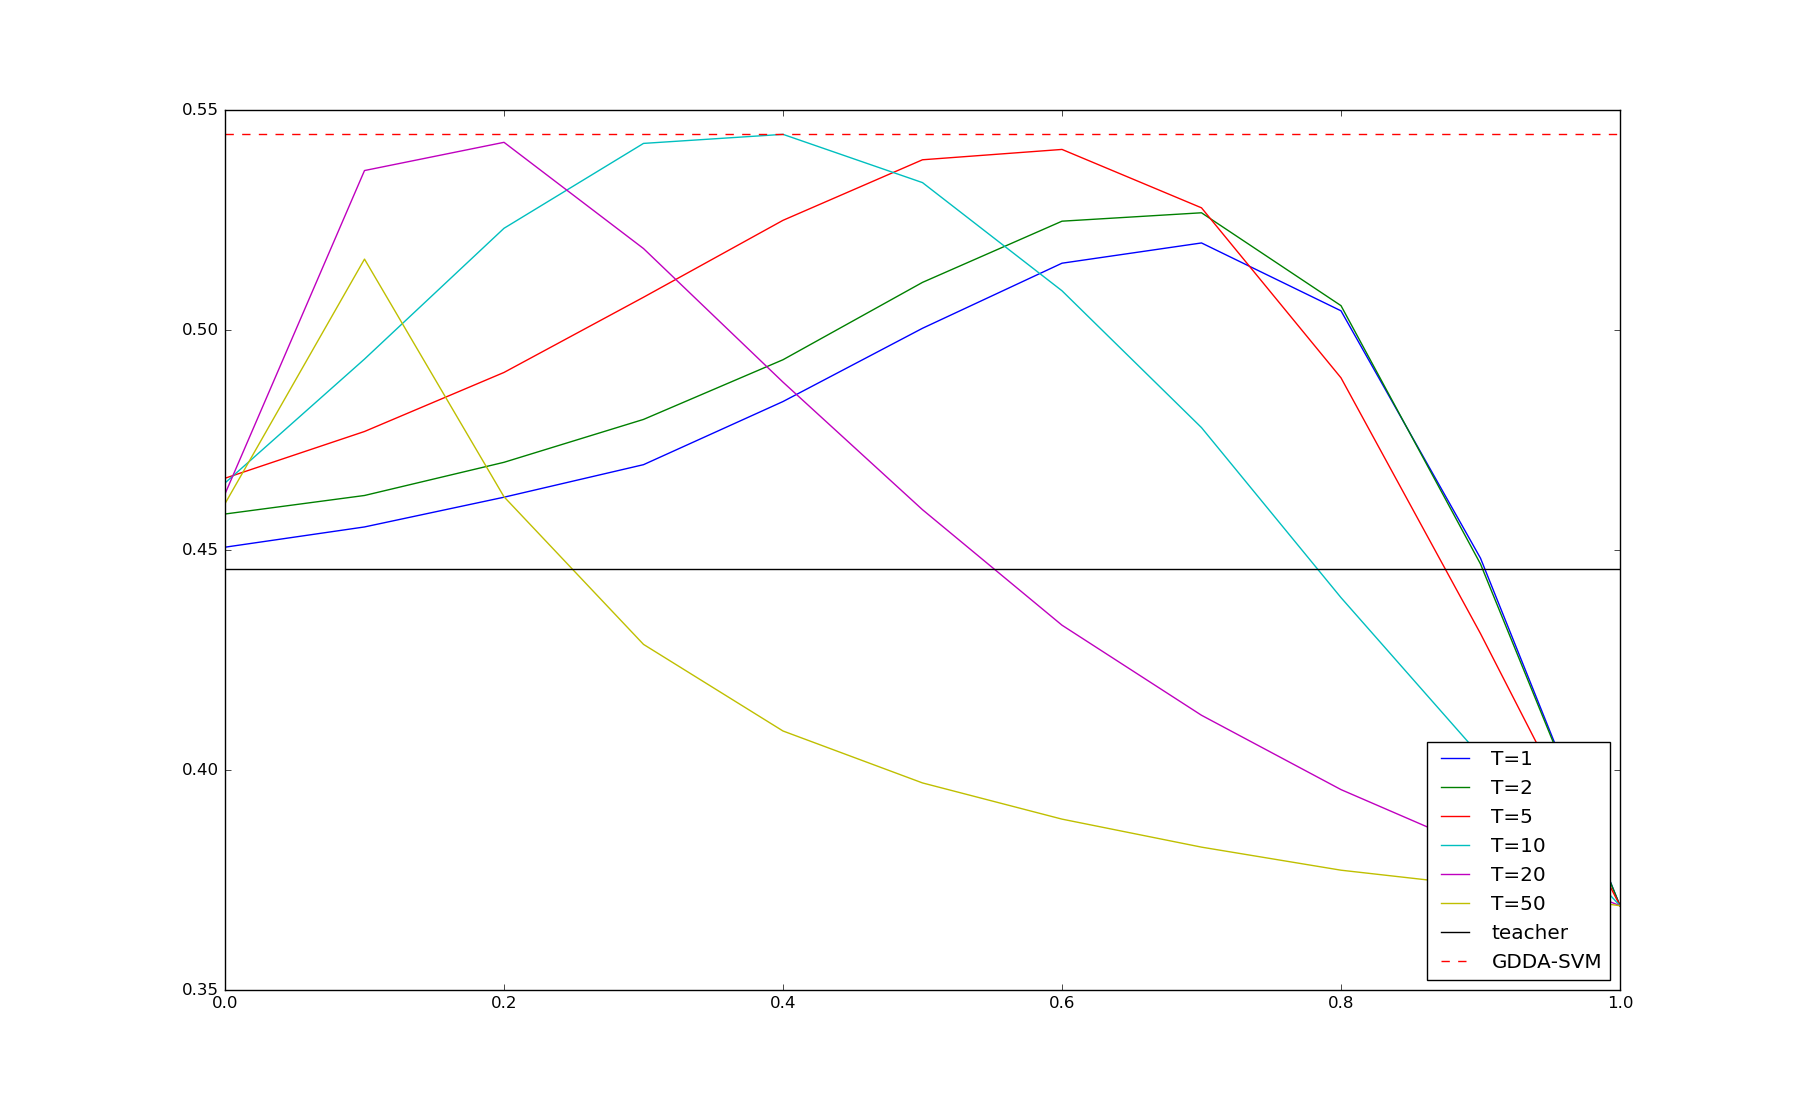
\includegraphics[width=0.45\textwidth]{figure/webcam4.png}}\\
\end{tabular}
\caption{Webcam $\rightarrow$ Amazon. Semi-supervised adaptation with one labeled instance per class.}
\end{figure}
\subsection{Multi-Source for Office datasets}
We transfer DSLR and Webcam to Amazon datasets with different settings:
\begin{figure}[h]
\centering
\begin{tabular}{cc}
\subfloat[5 unlabeled ]{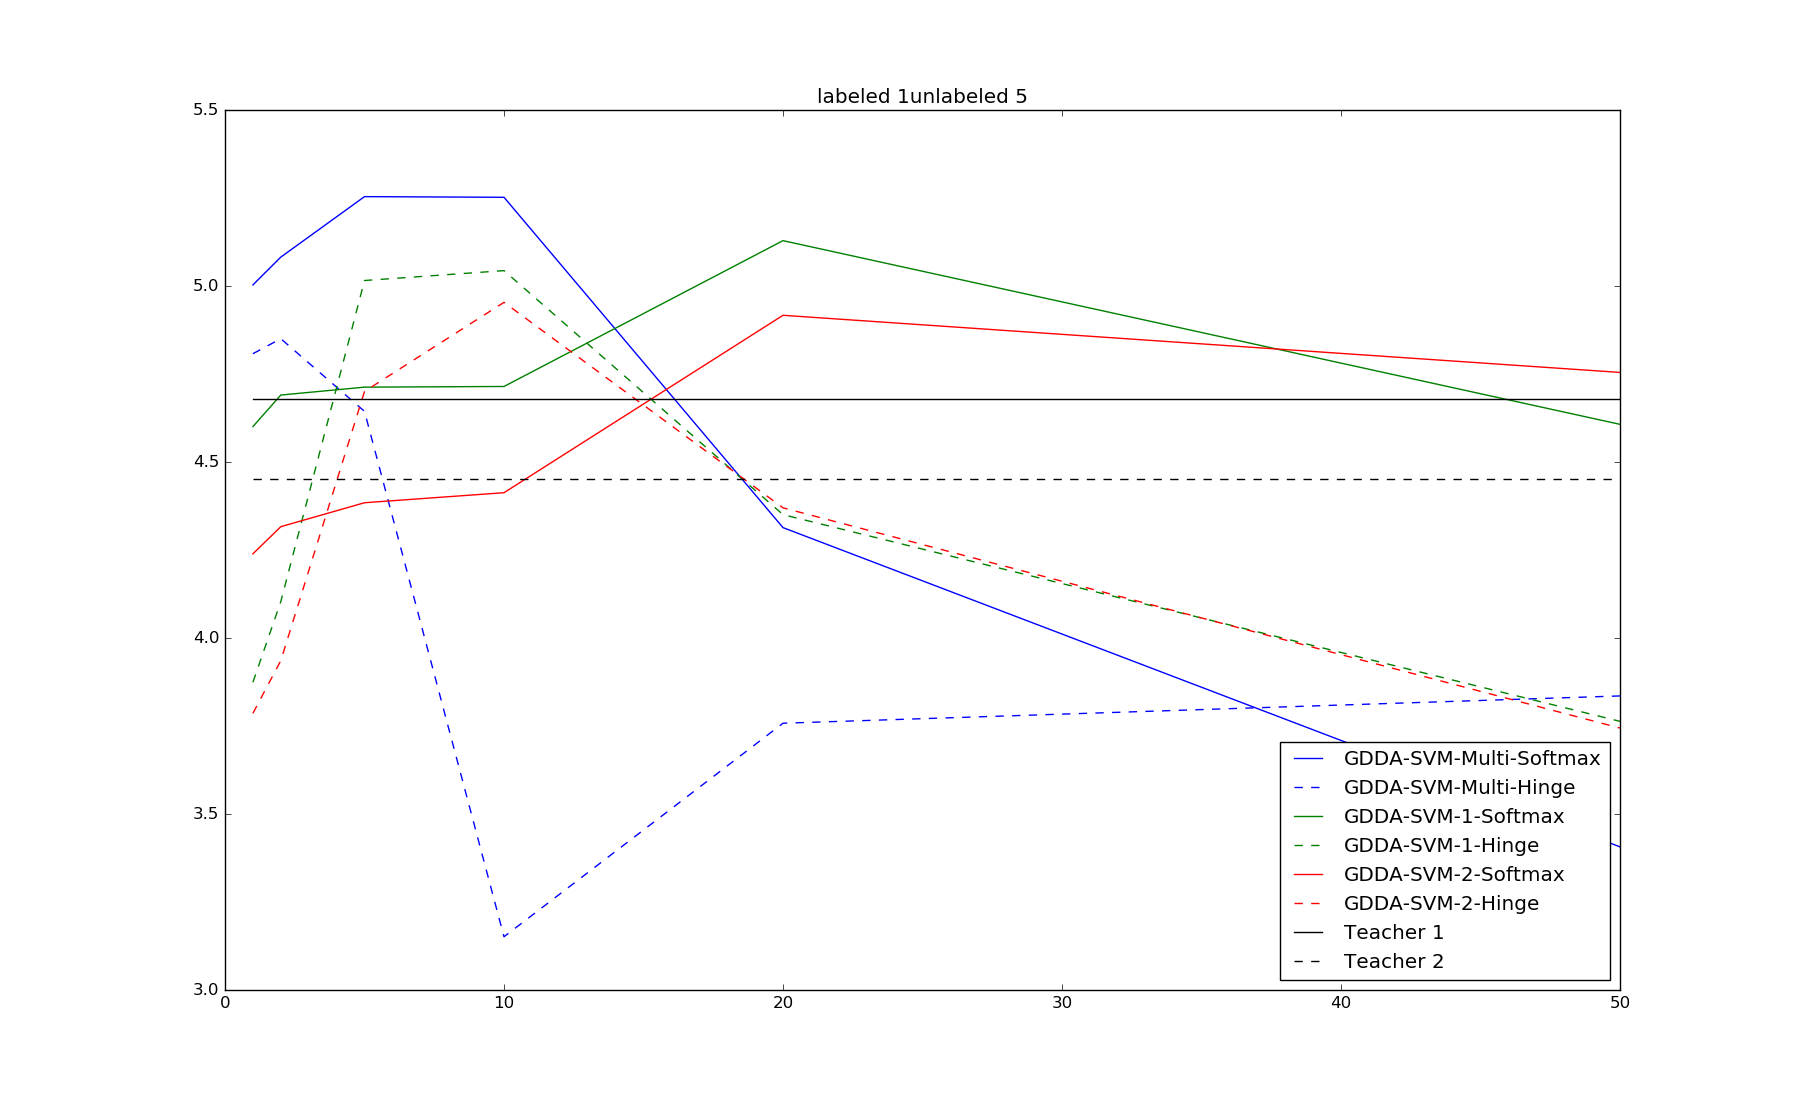
\includegraphics[width=0.45\textwidth]{figure/labeled1 unlabeled5.png}}&
\subfloat[10 unlabeled]{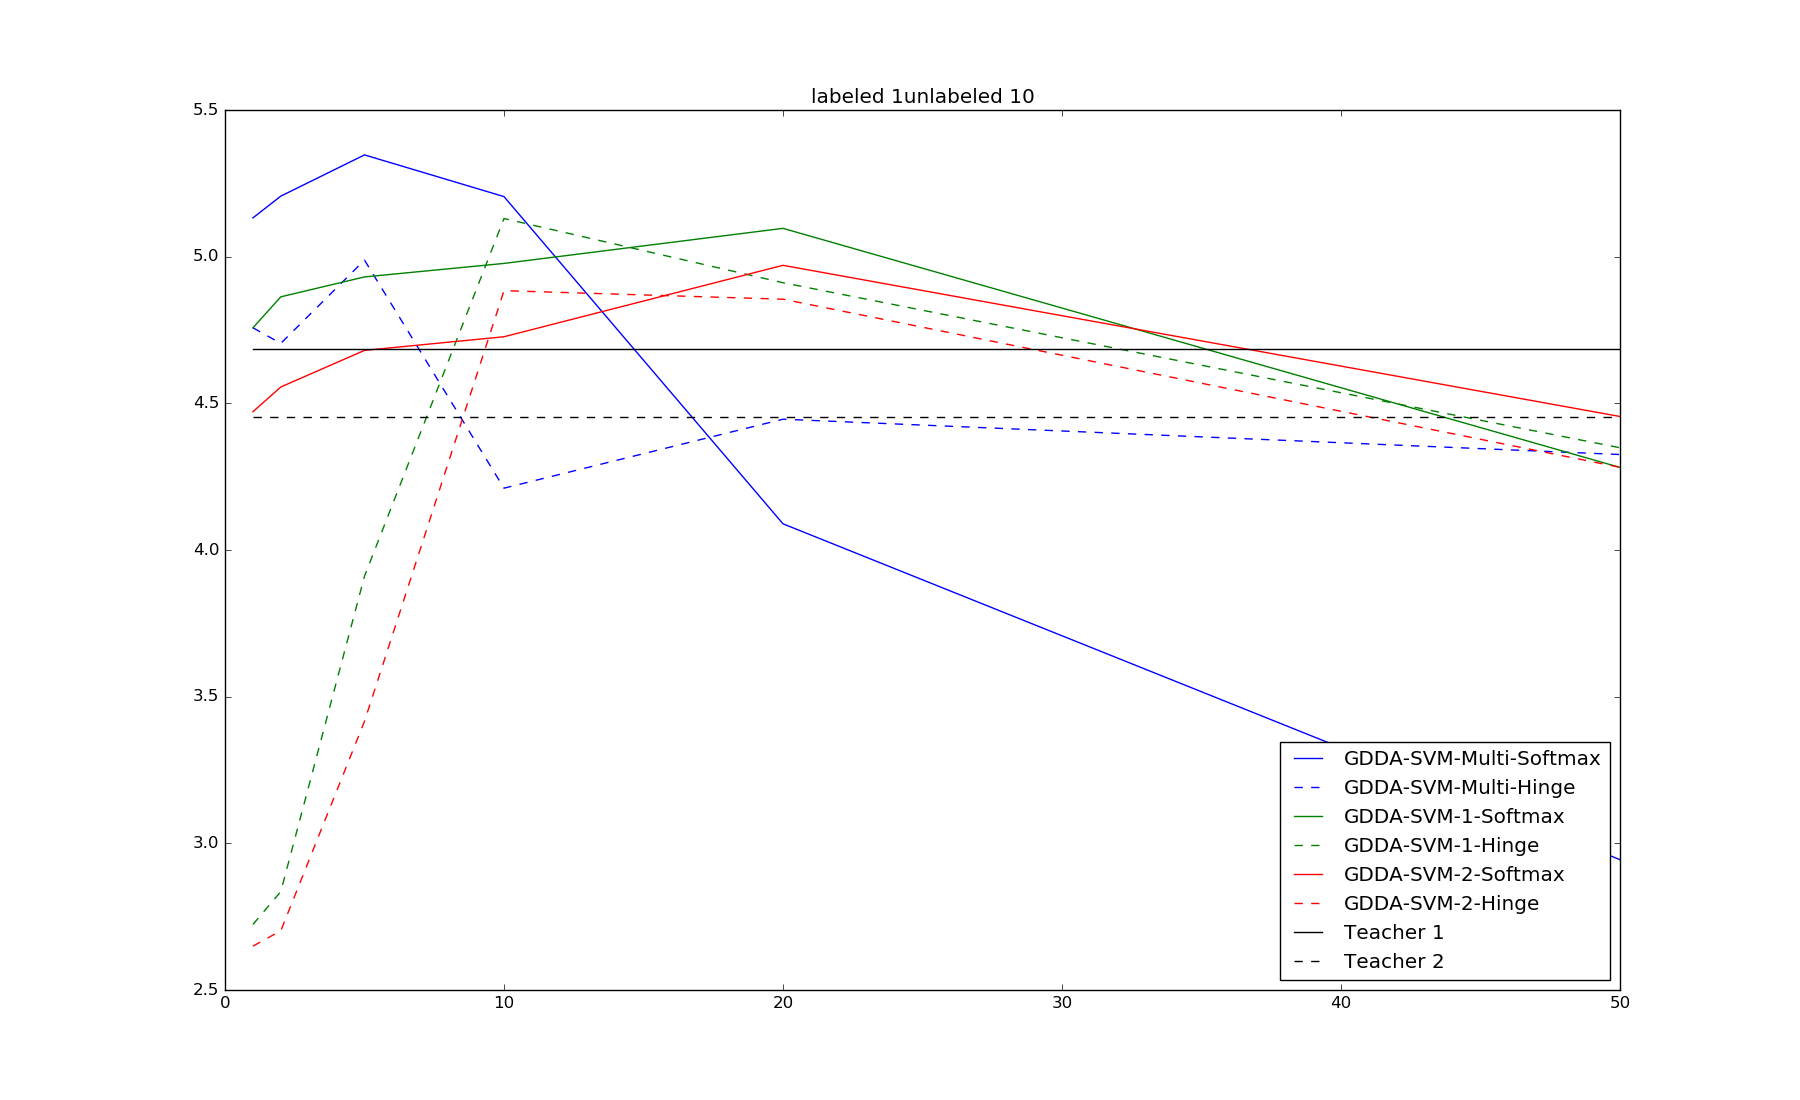
\includegraphics[width=0.45\textwidth]{figure/labeled1 unlabeled10.png}}\\
\subfloat[15 unlabeled]{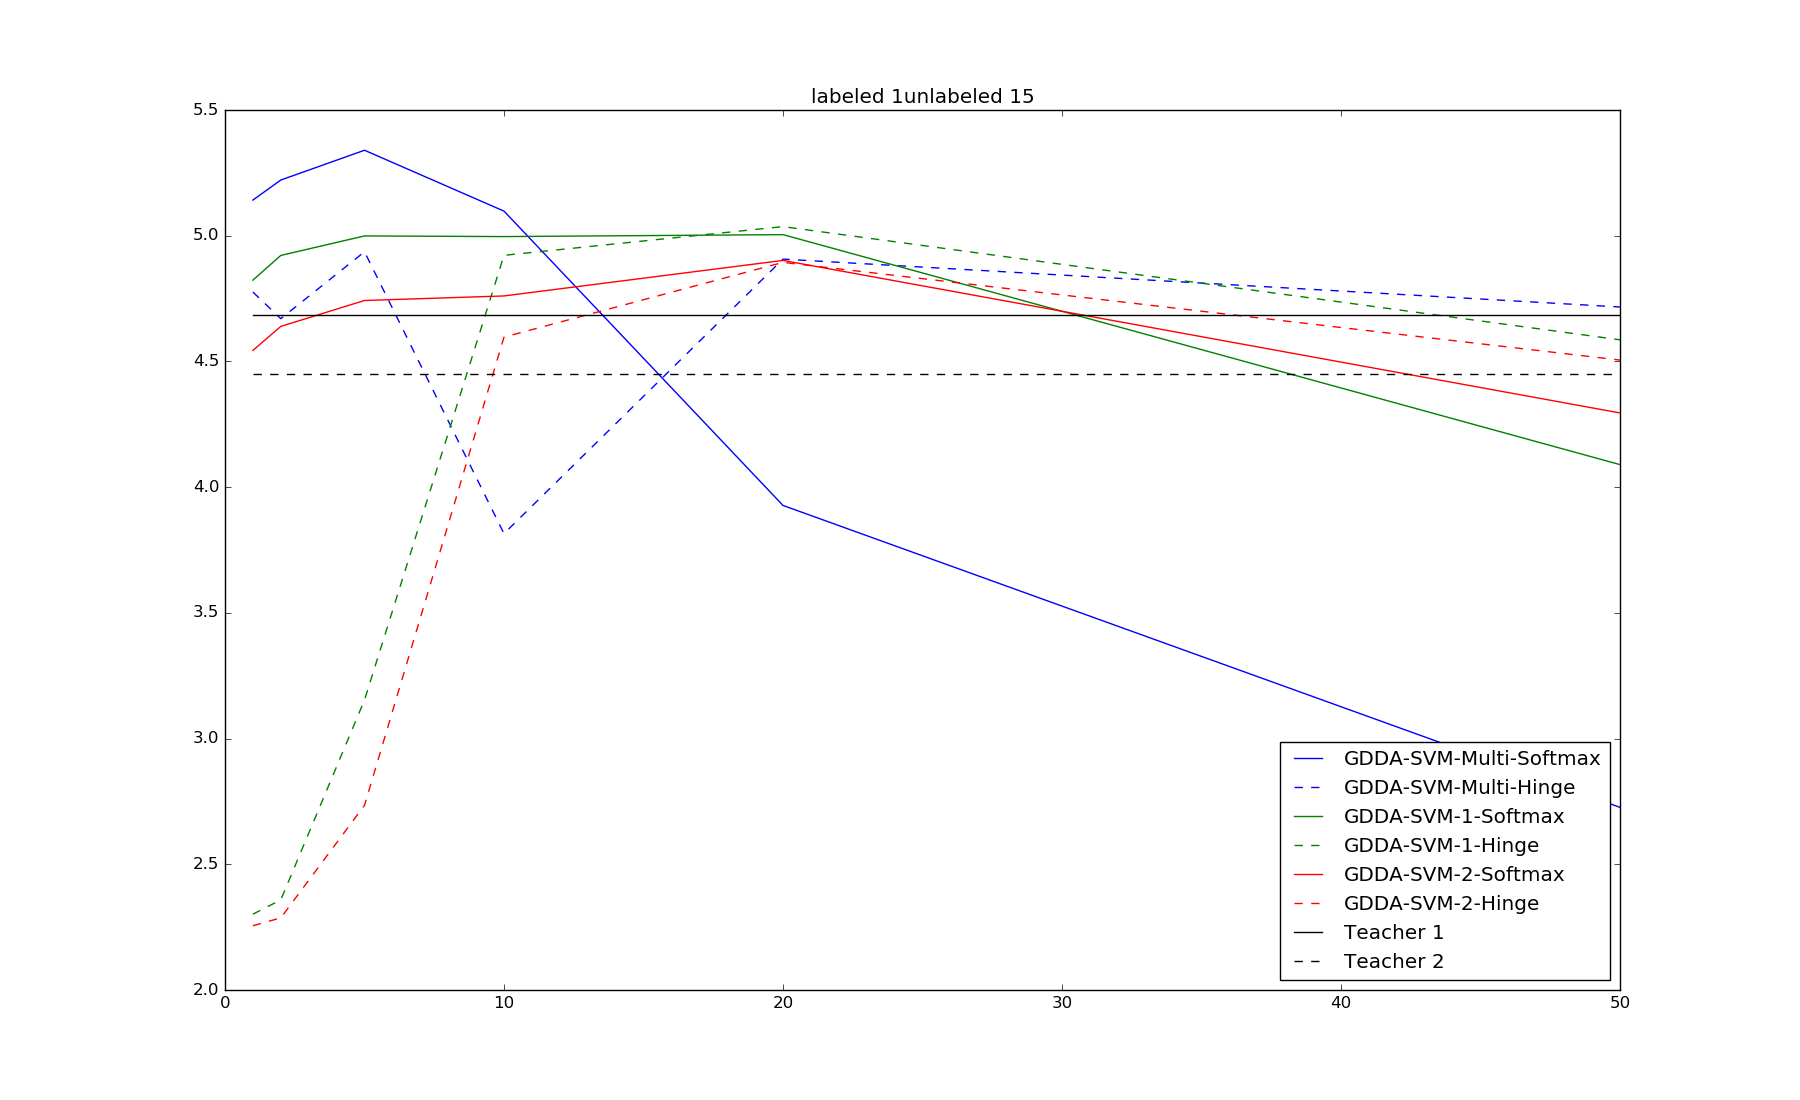
\includegraphics[width=0.45\textwidth]{figure/labeled1 unlabeled15.png}}&
\subfloat[20 unlabeled]{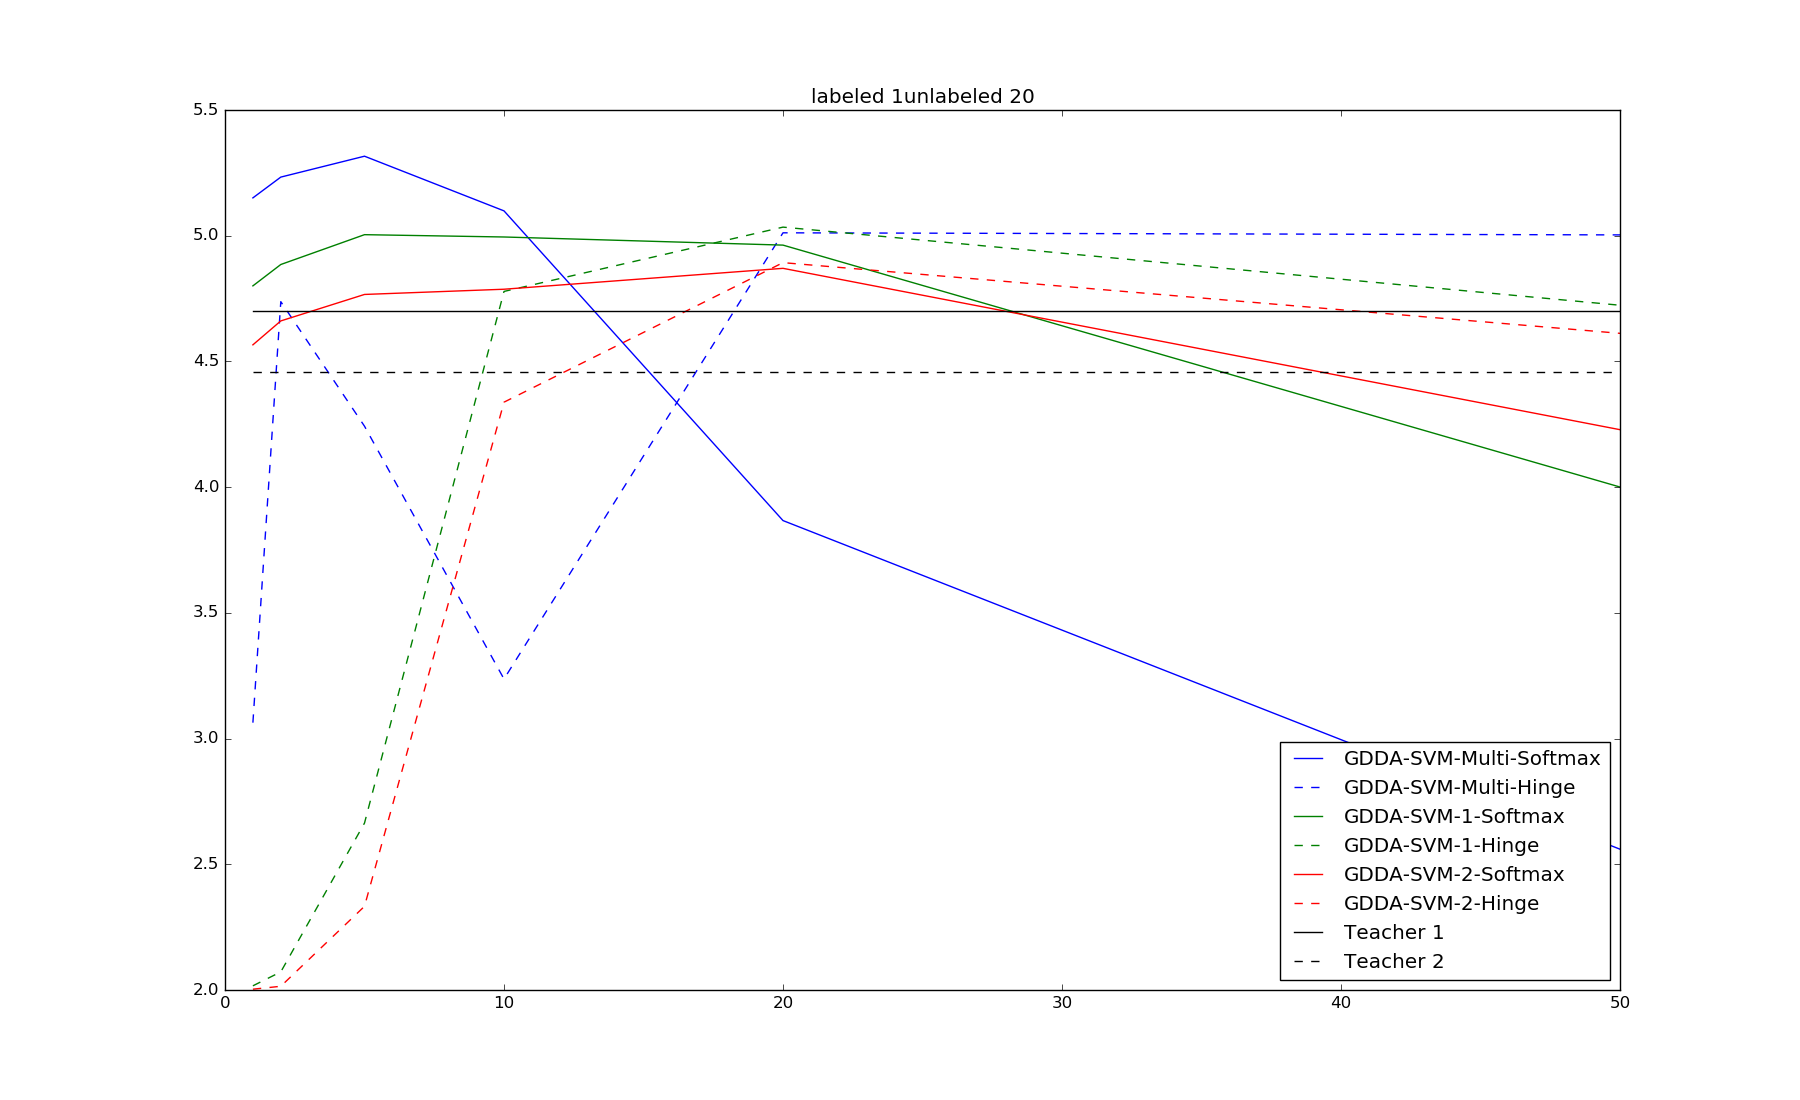
\includegraphics[width=0.45\textwidth]{figure/labeled1 unlabeled20.png}}\\
\end{tabular}
\caption{Webcam $\rightarrow$ Amazon. Semi-supervised adaptation with one labeled instance per class.}
\end{figure}




\section{Future works}
From current experiments we can see that GDDA can be a good framework for domain adaptation in single source scenario. We show that GDDA-SVM can fully exploit the knowledge from the source model. There are still a lot of work to be done within the GDDA-SVM framework:
\begin{enumerate}
\item Add experiments on heterogeneous data.(Ask the advice from Wei Yin) 
\item Add theoretical analysis on how the size of unlabeled data affect the performance of the target model. (Why increase the size of the unlabeled data can improve the performance at the beginning?)
\item Can we aggregate GDDA-SVM framework into the deep neural network to train a deep GDDA network? Currently, GDDAA-SVM tries to estimate the imitation parameter by solving a convex problem. How to effectively estimate the imitation parameter when it is integrated into a GDDA network. 
\end{enumerate}
\bibliographystyle{abbrv}
\bibliography{research}
\end{document}